% \documentclass[a4paper,10pt]{article}
 \documentclass[review,times,3p,10pt]{elsarticle}
\usepackage[utf8]{inputenc}

\usepackage{graphicx}
\usepackage{graphics}
\usepackage{enumitem}

\usepackage{epsfig}
\usepackage{subfigure}
\usepackage{tabularx}
\usepackage{amssymb}
\usepackage{amsmath}

\usepackage{colortbl}

\usepackage{enumitem}
% \usepackage{a4wide} %full page
\usepackage{fullpage}
\usepackage{hyperref}
\hypersetup{
  colorlinks   = true, %Colours links instead of ugly boxes
  urlcolor     = blue, %Colour for external hyperlinks
  linkcolor    = blue, %Colour of internal links
  citecolor   = red %Colour of citations
}

\usepackage{jabbrv}
\setlength{\bibsep}{1.0pt}
\bibliographystyle{myplainnat}
\usepackage{natbib}

\usepackage{amsmath,amssymb}
\usepackage{setspace}
\usepackage[scientific-notation=true]{siunitx} %VVV
\sisetup{round-mode = places, round-precision = 3} %VVV
\doublespacing

\usepackage{booktabs}
\usepackage{multirow}
\usepackage{url}

%  \usepackage{multirow}
 \usepackage[table,xcdraw]{xcolor}

% \usepackage{jabbrv}

\usepackage{blindtext}
\usepackage{todonotes}


 \RequirePackage{lineno} 

% \bibliographystyle{model2-names}
\biboptions{authoryear}

\newenvironment{lineq}
    {\begin{linenomath*}
    \begin{equation}
    }
    { 
    \end{equation} 
    \end{linenomath*}
    }


\newcommand{\dd}{\mathrm{d}}
\renewcommand{\vec}{\mathbf}
 \newcommand{\subscript}[2]{$#1 _ #2$}
 
 \newcommand{\norm}[1]{\left\lVert#1\right\rVert}

 \newcommand{\Lb}{\pazocal{L}}
 
\newcommand{\fs}{\footnotesize}
    \renewcommand{\arraystretch}{1.5}

\newcommand{\mich}[1]{{\color{magenta}{#1}}}

\journal{Computers \& Mathematics with Applications}

\begin{document}

\begin{frontmatter}



\title{Automated calibration methodology to avoid convergence issues during inverse identification of soil unsaturated hydraulic properties.}

\author[autor1]{Michal Kuraz}

\author[autor1]{Lukas Jac\v{c}ka}

\author[autor1]{Johanna Ruth Bl\"ocher}

\author[autor2]{Mat\v{e}j Lep\v{s}}



\address[autor1]{Czech University of Life Sciences Prague, Faculty of Environmental Sciences, Department of Water Resources and Environmental Modeling}

\address[autor2]{Czech Technical University in Prague, Faculty of Civil Engineering, Department of Mechanics}

\begin{abstract}
The single ring (hereafter SR) infiltration experiment is a standard and robust dynamic field experiment. The steady state part of this experiment is traditionally used for the identification of saturated hydraulic conductivity. In this contribution, we explore the possibility of extending the applicability of this experiment for evaluating the unsaturated hydraulic parameters from an unsteady part of this experiment for the top soil layer using inverse analyses of the governing flow motion equation.

The problem of SR infiltration is governed by the quasilinear Richards equation. We present a new scanning methodology to avoid convergence issues with the nonlinear operator, originating from difficult combinations of input parameters, which can be hard to avoid when automatically analyzing a broad parameter space. We validated our methodology with virtual infiltration problems for clay and sand, and applied it on real-world SR infiltration data. To evaluate non-uniqueness, local optima were identified and mapped using a modified genetic algorithm with niching.

Our results show the existence of multimodality in, both, the benchmark problems and the real-world problem. This is an important finding as local optima can be identified, which are not necessarily physical and also for systems that do not exhibit multimodal grain size distributions. The identified local optima were distinct and showed different retention and hydraulic conductivity curves. The most physical set of SHP could be identified with the knowledge of the saturated water content. 




%To evaluate non-uniqueness, local optima were identified and mapped using a modified genetic algorithm with niching.   
%We also discuss important issues regarding (i) the design of the numerical simulations and (ii) the influence of spatial and temporal discretization on the identified local optima.

\end{abstract}

\begin{keyword}
 single ring experiment \sep soil hydraulic properties \sep inverse modeling \sep Richards equation \sep convergence issues  \sep automatic calibration \sep computational issues in geosciences  

%% MSC codes here, in the form: \MSC code \sep code
%% or \MSC[2008] code \sep code (2000 is the default)

\end{keyword}

\end{frontmatter}

\linenumbers

\section{Introduction}%[lukas]
% -motivace

Soil hydraulic properties (hereafter SHP) are important for many hydrological models and engineering applications. The mountainous podzolic soil evaluated here is typical for the source areas of many major rivers in the Central European region. The top layer of the soil plays a key role in the rainfall-runoff process, because it is the top-soil that separates the rainfall into surface runoff and subsurface runoff. 


Due to the rocks present and the dense root system of the covering vegetation, and due to the possible extension of the representative elementary volume, it is often impossible to collect undisturbed samples of top-soil for laboratory measurements in order to obtain the SHP parameters~\citep{Jacka1}. The SHP of the topsoil are therefore very difficult to measure directly~\citep{Fodor, Jacka1}. 


 
\mich{In our study, we explore the applicability of the well-known single ring (hereafter SR) infiltration for evaluating the SHPs of the top soil from an unsteady part of this experiment.}
The SR infiltrometer is a widely accepted, simple, robust field method, which is able to measure the infiltration process, which affects the entire soil profile including the top-soil,  and can sample a relatively large volume (depending on the diameter of the ring)~\citep{Cheng,ReynoldsWD}.  The SR infiltration experiment is an in situ experiment, which does not require soil samples to be collected, so the porous medium is kept relatively undisturbed. With the widely-used ring diameter of 30~cm, the affected porous media is far more representative than any soil sample we were able to collect. The top-soil can also be measured (with some alteration of the surface) using other well-known field infiltration methods, e.g. the tension infiltrometer or the well permeameter  \citep{AnguloJaramillo,ReynoldsWDGP}. 

The Richards equation~\citep{richards} describes flow in variably saturated porous media. In order to model environmental processes and engineering applications with the Richards equation knowledge of the SHP is essential. SHP can be summarized by the soil water retention curve and soil hydraulic conductivity curve. In this contribution, the SHP are parametrized with the frequently used Mualem-van Genuchten model~\citep{vangenuchten}. We refer to this model as REVG.



% with VG parameters governing retention curve and unsaturated hydraulic conductivity, where the SHP are typically described by VG parameters, saturated hydraulic conductivity and residual and saturated water content.
% And so 
%  it is expected that the Richards equation can be used for inverse analysis of the of SHPs the top-soil on the basis of the measured unsteady infiltration data. It is apparent that the both unknown saturated and residual water content in case of an absence of the water content experimental data yields non-unique solution of Richards equation inverse model, the residual water content should be excluded from the identification, see~\citep{mous1993}.




 
The identification of SHP from transient infiltration experiments has been a subject of numerous publications in past decades \citep{simunek-infiltr2shp, infiltr2shp, simunek2-infiltr2shp, XU201234, BAGARELLO201770,  hess-Younes-2017}.  \cite{simunek-infiltr2shp} reported a close correspondence between the SHP obtained from the inverse modeling of dynamic transient infiltration experiments with those obtained from steady-state laboratory experiments, where the uniqueness of the inverse model was preserved by considering the dynamically changing pressure head, water content and even tracer concentration.

The non-uniqueness of the REVG inverse model is already a very well-known issue, and has been described by a number of publications over the last decades~\citep{kool1985, mous1993, ihlwang2003, beven2003-uncertain,Kowalsky04,Nakhaei, Kamali,pena17}.
\cite{mous1993} defined criteria for model identifiability based on the sensitivity matrix rank, however numerical computation of the sensitivity matrix, which is defined by the derivatives of the objective function, often involves difficulties in managing truncation and round-off errors.
\cite{beven2003-uncertain} demonstrated on a real world case study of Sherwood Sandstone Aquifer that many different SHP parameters of macroscopic media can represent the layered unsaturated zone and provide acceptable simulations of the observed aquifer recharges.  \cite{mous1993} explained that in case of the absence of water content data, the residual water content should be excluded from the identification to avoid non-uniqueness. However, \cite{beven2003-uncertain} used
a non-unique definition where both the unknown residual and saturated water content were considered.
The definition of a unique inverse function for identification of macroscopic media was treated in~\citep{zou200126}, where the recommended approach was to assemble the objective function from transient data of the capillary pressure and from the steady state water content data. 

A challenging issue is the treatment of the nonlinear operator of the Richards equation. \cite{beven2003-uncertain} reported that 56\% of the simulations were rejected during Monte Carlo simulations on a wide range of parameters, because of convergence problems. 
Their study did not mention explicitly why. \mich{ We assume that these convergence issues originated from 
 difficult combinations of input parameters, which can be hard to avoid when automatically analyzing a broad parameter space. }


The following questions arise: 
\begin{itemize}
\item How can convergence issues be avoided, especially when the parameter range is wide? 
\item Is it possible to approximate the unsteady SR infiltration experiment using the REVG model, where the only unknown parameters represent the thin topsoil layer, by a unique set of parameters? 
\item If not, are all parameters vulnerable to non-uniqueness?
\end{itemize}

To answer these questions we employed a new calibration methodology.

 \mich{The purpose of this paper is to answer the given research questions. The first part of the paper presents the real world background of the analyzed SR infiltration data. However, for the demonstrative purposes of this contribution, we have significantly reduced this data part, and only the mean values are analyzed here. Data error propagation and further statistical analyzes are beyond the scope of this paper. The major part of this paper is focused on a design of calibration methodology for the SR experiment. We start with derivation of the governing equation for this class of problems. Numerical issues with convective term as well as the domain shape restrictions and boundary condition setup is given. Then we continue with a synthetic inverse problem with known exact solution, where we try to identify SHPs from cumulative fluxes across the Dirichlet boundary, which is an analogy to the infiltration experiment.  Further we propose calibration methodology, where we presume smooth and continuous convergence properties of the inverse problem, which is represented by a discrete and linearized analogue of the Richards equation, for both nonlinear operator stopping criterion, temporal discretization and spatial discretization. Based on the results from the synthetic problem, we are already aware of multimodality of this inverse model. In order to obtain a unique solution we employ an expert knowledge as a final decision making criterion, since each parametric set comes with a distinct saturated water content (herafter $\theta_s$) value. Although we can't measure the exact value of $\theta_s$ for the top soil layer, since it is impossible to collect undisturbed samples with representative volume size, and so removing this parameter from the inverse model is questionable, acceptable ranges of $\theta_s$ form a part of the expert knowledge. 
 
 In general, the proposed novel calibration methodology can be applied  for inverse analyses of quasi-linear parabolic differential equations, such as Richards equation problems.
 }




\subsection{Comment on system of units applied in this manuscript}

Due to spatial and temporal scales of all model scenarios evaluated in this manuscript, instead of the base SI units we preferred to make use of {\it non-SI units  accepted for use with the SI}. The length [L] will be always given in [cm], and the time [T] will be always given in [hrs].






\section{Methodology}% [lukas a michal]
\label{metodo}


This section is divided into two parts. The first part, section~\ref{assamb}, is focused on assembling the experimental data, which were later used as input for the inverse model. The site description, the reconstruction of the parameters of the SHP for the lower profiles, and the processing of the experimental data is given.   

The second part of the methodology covers issues in the REVG inverse model. Section~\ref{goveq} derives governing equations and is given together with notes on the numerical stability of the REVG model for rotational symmetric problems.
Section~\ref{bccond} discusses issues in creating the domain scheme and selecting appropriate boundary conditions, since it is not always easy to find an agreement between the mathematical model setup and  physical interpretation. Section \ref{objdef} concludes with a description of the construction of the objective function, and the methodology of the automatic calibration. 


\mich{\subsection{Comment on soil hydraulic parameters}
\label{shpdescr}

\linelabel{line:shp} The soil hydraulic parameters (SHP) studied in this contribution refer to hydraulic properties of the porous medium under variably saturated state. Using the model by~\cite{vangenuchten} the following SHP are studied in this contribution
\begin{description}
\item[$\alpha$] -- inverse of air entry value [L$^{-1}$]
\item[$n$] -- pore size distribution parameter [-]
\item[$\theta_s$] -- saturated water content [-]
\item[$K_s$] -- saturated hydraulic conductivity [L.T$^{-1}$]
\item[$S_s$] -- specific storage [L$^{-1}$]
\end{description}
A detail description on $K_s$ and $S_s$ parameter is given by~\cite{bear1979}, and a detail description on parameters $\alpha$, $n$, and $\theta_s$ is given by~\cite{vangenuchten}.}




\subsection{Obtaining the input data for the inverse problem}
\label{assamb}



\subsubsection{Site description and assembling the experimental data}%[lukas]
\label{site}

\label{povodi}

\mich{In this section a brief description of the conducted experiments is given. Since this contribution is focused on calibration methodology, we will significantly reduce the experimental data analyses. Complete description of this experiment including statistical analyses of the experimental data is given in~\citep{jacka-site}.
}


The study site was located in the \v{S}umava National Park, \mich{Czech Republic},\linelabel{line:marker} and has been described by \cite{Jacka1}. The location of the site in a map of Modrava 2 catchment is presented by \cite{Jacka2}.
The soil profile is described by four different layers as seen in figure~\ref{experiment}. 
\mich{Series \linelabel{line:gw} of tension meter measurements of the top soil layer have been conducted on the site. The average soil suction head was estimated at 280~cm. If we further assume hydrostatic (no-flow) initial condition, then the average groundwater table can be roughly estimated at 280~cm below the surface. We are aware, that this assumption is a subject to strong uncertainty. In the real world the soil suction head distribution is almost never hydrostatic (especially for this relatively humid mountainous region). And so the estimated groundwater table is rather an overhead limit, which is already a significantly distant from the top-soil layer. With such hydrogeological configuration the effect of groundwater on infiltration experiment is expected to vanish. }





\mich{The SHP of the lower layers were identified by~\cite{Jacka1}, and are presented in table~\ref{tab_SHP}. }






 


%%%%%%%%%

%The estimated SHP for the lower horizons below the top soil are depicted in table~\ref{tab_SHP}.

\begin{table*}[ht]
\begin{center}
\caption{Soil hydraulic properties for the lower horizons.}
\fs
\begin{tabular}{c | p{2cm} | c c c c c}
\toprule
horizon &  GP experiment sites  & $\theta_s$ [-] & $\alpha$ [cm$^{-1}$]& $n$ [-]& $K_s$ [cm.hrs$^{-1}$] & $S_s$ [cm$^{-1}$] \\ \hline
E & 28 &  0.46 & 0.046 & 1.741 & 1.584 & 0\\
Bhs + Bs & 19  &0.47&  0.022 & 1.450 & 0.540 & 0\\
C & 8 & 0.50 & 0.035 & 4.030 &  3.060 & 0 \\
\toprule
\end{tabular}
\label{tab_SHP}
\end{center}
\end{table*}




 


 \begin{figure}
\centering
\rotatebox{90}{
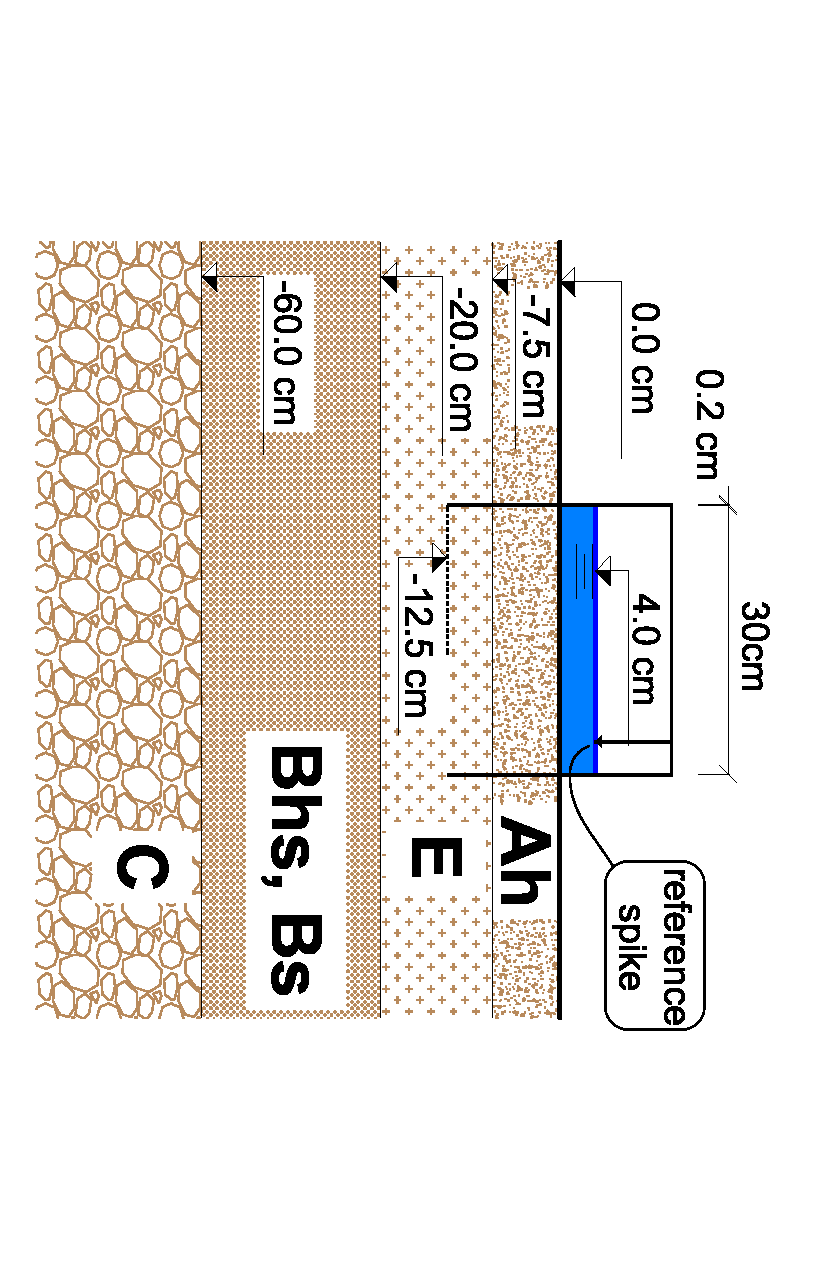
\includegraphics[height=7.5cm]{valec-exp.pdf}}
 \caption{Scheme of the single ring infiltration experiment and the soil layers. }
 \label{experiment}
\end{figure}



The experimental setup of the SR experiment was as follows. A steel ring 30~cm in inner diameter, 25~cm in length, and 2~mm in thickness was inserted into the soil to a depth of 12.5~cm, see figure~\ref{experiment}. The depth of ponding was kept approximately at a constant level defined by a reference spike, which was placed 4~cm above the surface of the soil. The average experiment duration was 60~minutes.


 \mich{For a simplicity and demonstrative purposes of our methodology,  the experimental data will be represented  by a single average curve, which has been already constructed by~\cite{jacka-site}. 
\cite{jacka-site} has constructed the representative infiltration curve on the basis of 
 the Swartzendruber equation~\citep{Swartzendruber}, which states that
\begin{lineq}
I(t)=\frac{c_0\left(1-\exp\left(-c_1\sqrt{t}\right)\right)}{c_1}+c_2t,
\label{vyhlaz}
\end{lineq}
where $I$ is the cumulative infiltration [$L$], and $c_{0,1,2}$ are parameters. The Swartzendruber model 
describes one-dimensional infiltration into a homogeneous medium, and is therefore not sufficient here. The Swartzendruber model was  considered as an  interpolating function.
A statistical description of the Swartzendruber parameters, such as standard deviation, mean value, parameter variability, and their fitting quality is given in~\citep{jacka-site}, see datasets collected on site 3. According to this data paper the representative mean values are as follows: $c_0 =5.130$~cm.hrs$^{-0.5}$, $c_1 = 1.13 \times 10^{-1}$~[-], and $c_2 = 1.858$~cm.hrs$^{-1}$. This parameter set together with \eqref{vyhlaz} and with the simplified assumption of error free data was used here to represent the input infiltration curve  for demonstrating the 
 calibration methodology proposed in this paper.
}







\subsection{Mathematical model of the field infiltration experiment -- governing equation}%[michal]
\label{goveq}


The field infiltration experiment is characterized by variably saturated conditions. The flux in porous media under variably saturated conditions can be expressed by the Darcy-Buckingham law~\citep{buckingham} \begin{lineq}\label{darcybuck}\vec{q} = -\mathbf{K}(\theta) \nabla H,\end{lineq} where $\vec{q}$ is the volumetric flux [L.T$^{-1}$], $H$ is the total hydraulic head [$L$] defined as $H=h+z$, where $h$ is the pressure head [$L$], $z$ is the potential head [$L$], $\theta$ is the water content [-], and $\mathbf{K}(\theta)$ is the unsaturated hydraulic conductivity  [L.T$^{-1}$]; in general it is a  second order tensor. The relation $\theta(h)$ is referred to as the retention curve~\citep{vangenuchten}.

The geometry of the flow is inherently three-dimensional, but the domain dimension can be reduced by considering the axisymmetric geometry. The law of mass conservation  for incompressible flow in cylindric coordinates is expressed as ~\citep{bear1979}.
\begin{lineq}
\label{conti}
-\frac{\partial V}{\partial t} = \frac{\partial q_r}{\partial r} + \frac{q_r}{r} + \frac{\partial q_{\alpha}}{\partial \alpha} + \frac{\partial q_z}{\partial z} ,
\end{lineq}
where $V$ is the volume function [-],  $r$ is the radial coordinate, $\alpha$ is the angular coordinate,  $z$ is the vertical coordinate, and $q_{r, \alpha, z}$ is the  volume flux [L.T$^{-1}$]. The ring infiltration experiment is characterized by rotational symmetric flow, so the angular derivative vanishes. Then the governing equation for  variably saturated and rotational symmetric flow is obtained by substituting the flux in \eqref{conti} by the Darcy-Buckingham law~\eqref{darcybuck}. Together with the consideration of linear elasticity (expressed by specific storage $S_s$) for a porous medium the variably saturated axisymmetric flow in isotropic media is governed by
\begin{lineq}
\label{richaxi}
\left(\frac{\dd \theta}{\dd h} + S_s\frac{\theta(h)}{\theta_s} \right) \frac{\partial h}{\partial t}  =  \frac{\partial K(h) \frac{\partial H}{\partial z}}{\partial z} + \frac{\partial K(h) \frac{\partial H}{\partial r}}{\partial r} + c(\vec{x})\frac{\partial H}{\partial r},
\end{lineq}
where $S_s$ is the specific storage [L$^{-1}$], $\theta_s$ is the saturated water content [-],  $c(\vec{x})$ is the coefficient of the convection for $r$ coordinate [T$^{-1}$], which is explained below, and the vector $\vec{x}$ is a vector of the spatial coordinates $\vec{x}=\left( \begin{smallmatrix} r \\ z \end{smallmatrix} \right)$.

 \begin{figure}
\centering
\rotatebox{90}{
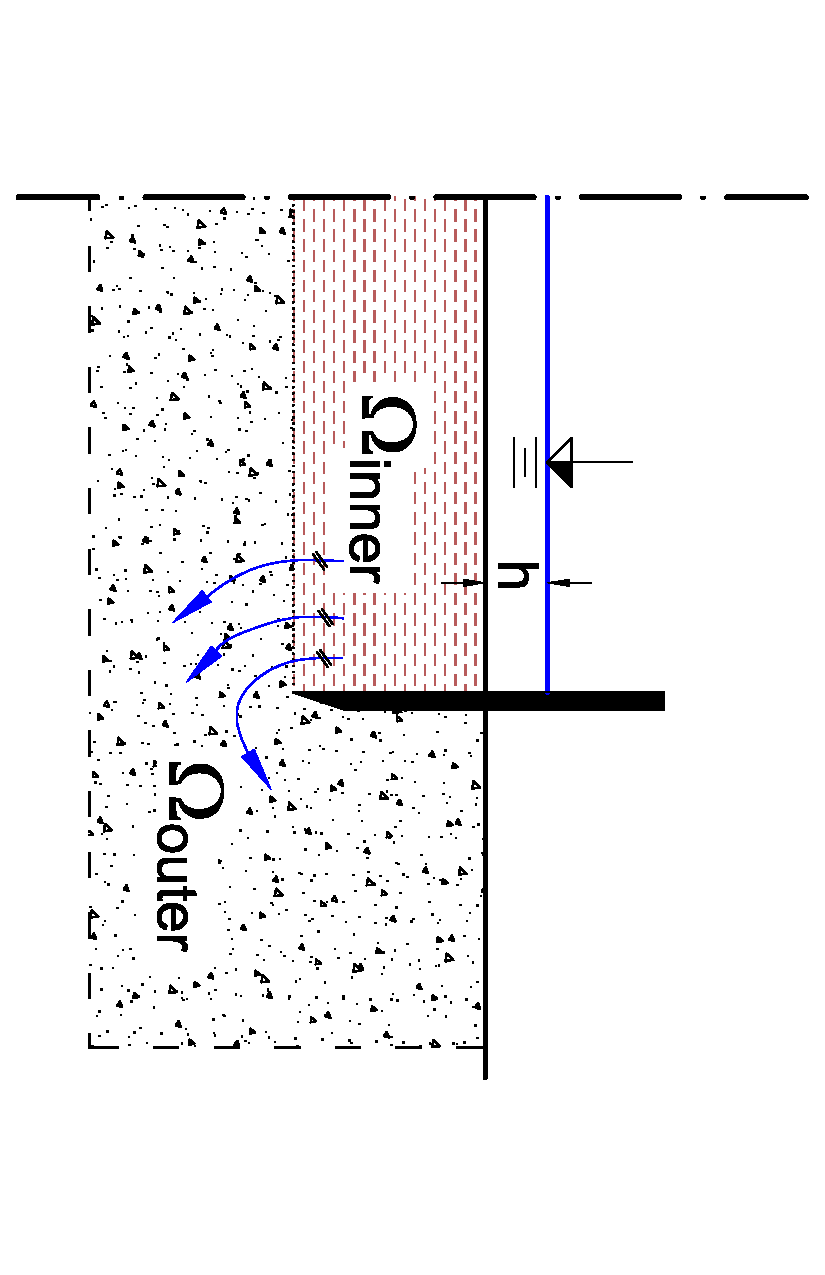
\includegraphics[height=7.5cm]{valcovazk.pdf}}
 \caption{Scheme of the flow domain and the streamlines of infiltration experiment. }
 \label{valecproudy}
\end{figure}

If we consider the model of the infiltration experiment depicted in figure~\ref{valecproudy} with the entire flow domain $\Omega=\Omega_{inner} \cup \Omega_{outer}$, where $\Omega_{outer}$ is the flow domain outside the infiltration ring and $\Omega_{inner}$ is the flow domain within the infiltration ring, exactly as depicted in figure~\ref{valec}. It is then apparent that the streamlines inside subdomain $\Omega_{inner}$ are parallel, but the streamlines outside the infiltration ring (inside $\Omega_{outer}$) are only axisymmetric. The convection coefficient $c(\vec{x})$ is then defined as follows
\begin{lineq}
\label{convect}
c(\vec{x}) = \begin{cases}
	     0 , \quad &\forall \vec{x} \in \Omega_{inner} \\
	     \frac{1}{r}K(h) , \quad &\forall \vec{x} \in \Omega_{outer}.
	    \end{cases}
\end{lineq}
Note that we should avoid using the coordinates, where $r=0$.


\subsection{Domain setup}%[michal]
\label{sec:bccond}







\subsubsection{Initial and boundary condition setup}
\label{ibc}

 \begin{figure}
\centering
\rotatebox{90}{
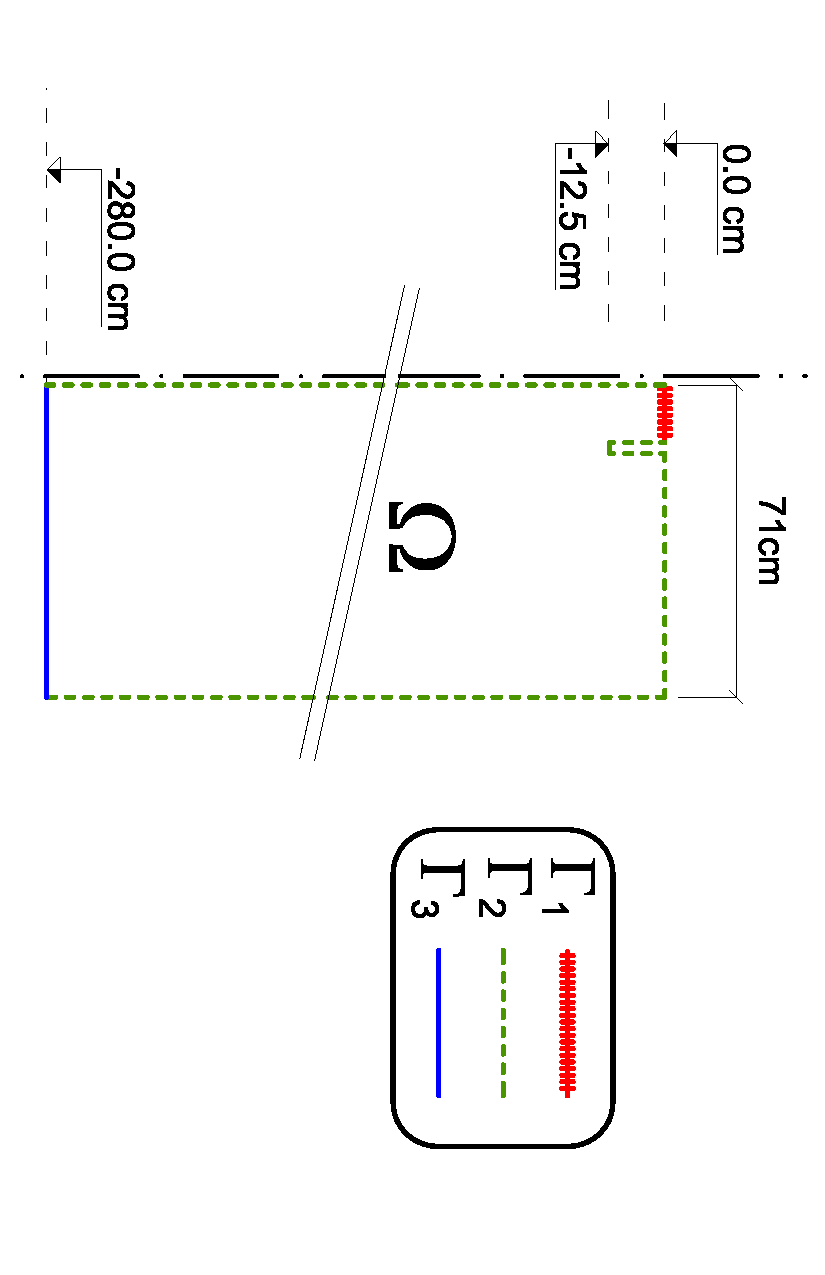
\includegraphics[height=8cm]{schemabc.pdf}}
 \caption{Scheme of the computational domain geometry and the domain boundaries.}
 \label{valecbc}
\end{figure}

\linelabel{line:ibc} \mich{The computational domain scheme is depicted in figure~\ref{valecbc}.}
The initial condition was assumed as a steady state  solution  of \eqref{richaxi} with the boundary $\Gamma_1 \cup \Gamma_2$ assumed as a no-flow boundary -- thus the entire domain $\Omega$ was considered to be in a hydrostatic state. The initial condition states that 
\begin{lineq}
\label{icond}
	H(x) = -280.0 \; \mbox{cm}; \quad \forall x \in \Omega,
\end{lineq}
and thus $\frac{\partial h}{\partial z} = -1$.

The left hand side boundary was located at $r=2$~cm, and the right hand side boundary was located at a distance $r=73$~cm, which is 60~cm from the infiltration ring. \mich{The reasons for such position of the left hand side boundary will be explained in the section below.}

 The location of the top boundary was natural -- the soil surface. Inside the ring, a Dirichlet condition defines the ponding depth; outside the infiltration ring a Neumann condition defines the no-flow boundary. The depth and definition of the bottom boundary was more problematic. We consider following commonly used options:
\begin{itemize}
\item the no-flow boundary (Neumann)
\item the free drainage boundary (Neumann)
\item the groundwater level - zero pressure head (Dirichlet)
\end{itemize}
It is apparent that the wetting front originating from our infiltration experiment affects the soil column only to a certain depth. Defining the Neumann no-flow boundary at a sufficient depth would probably not have a significant effect on the cumulative flux at the top Dirichlet boundary. At the same time, the only physically acceptable location of the no-flow boundary is the impermeable layer. The second option -- the free drainage boundary -- would be completely incorrect for any depth, because we consider the initial condition to represent a hydrostatic state, and so \begin{lineq} \frac{\partial h}{\partial z}(x) = -1, \quad \forall x \in \Omega .\end{lineq} The free drainage boundary condition, which is defined as
\begin{lineq}
\frac{\partial h}{\partial \vec{n}}(x) = 0, \quad \forall (x,t) \in \Gamma_{\mbox{\footnotesize free drainage}} \times [0,T).
\end{lineq}
is in a conflict with the initial condition (since the outer normal vector $\vec{n} = \left(\begin{smallmatrix} &0 \\ -&1 \end{smallmatrix} \right)$), and produces extra computational costs. The computed fluxes produced at the bottom boundary in the beginning of the simulation with such a boundary setup, originates from the initial and boundary condition mismatch, and has no physical meaning.

Physically correct boundary conditions for the bottom boundary is either the Neumann no-flow boundary at the impermeable layer or Dirichlet boundary both at the groundwater table. We chose a constant Dirichlet boundary condition. \mich{The minimum depth} of the groundwater table was estimated at -280~cm below the surface, \mich{see the explanation given in section~\ref{site},} and  we assume that the water table remains constant during the experiment. With this particular setup the domain became extremely narrow and deep, see figure~\ref{valec}.\mich{ \linelabel{line:dbc} The potential implication of this assumption is that the groundwater aquifer adsorbs the entire infiltrated amount without affecting its volume. In theory, this assumption is non-physical. However, for a short  experiment, such as the evaluated infiltration experiment, when the infiltrating wetting front within the simulation time even doesn't reach a vicinity of the groundwater aquifer, and  with the consideration, that the infiltrated amount is  negligible in comparison to the   aquifer volume, this assumption becomes acceptable.}





The locations of the domain boundaries are depicted in figure~\ref{valecbc}. The boundary conditions are specified as follows (with the reference level $z=0$ located at the top boundary)
\mich{\begin{lineq} 
\label{bccond}
\begin{split}
h(x,t) &= 4 \; \mbox{cm} \Rightarrow H(x,t) = 4 \; \mbox{cm}; \\ &\forall (x,t) \in \Gamma_1 \times [0,T), \\
\norm{\frac{\partial H}{\partial \vec{n}}}_2 &= 0; \, \forall (x,t) \in \Gamma_2 \times [0,T), \\
h(x,t) &= 0  \; \mbox{cm}  \; \Rightarrow \; H(x,t) = -280.0  \; \mbox{cm}; \\ &\forall (x,t) \in \Gamma_3 \times [0,T).
\end{split}
\end{lineq}}
where $T$ is the simulation end time [T], and $\vec{n}$ is the outer normal boundary vector.

\subsubsection{Domain shape restrictions}
\label{shaperestr}

 \begin{figure}
\centering
\rotatebox{90}{
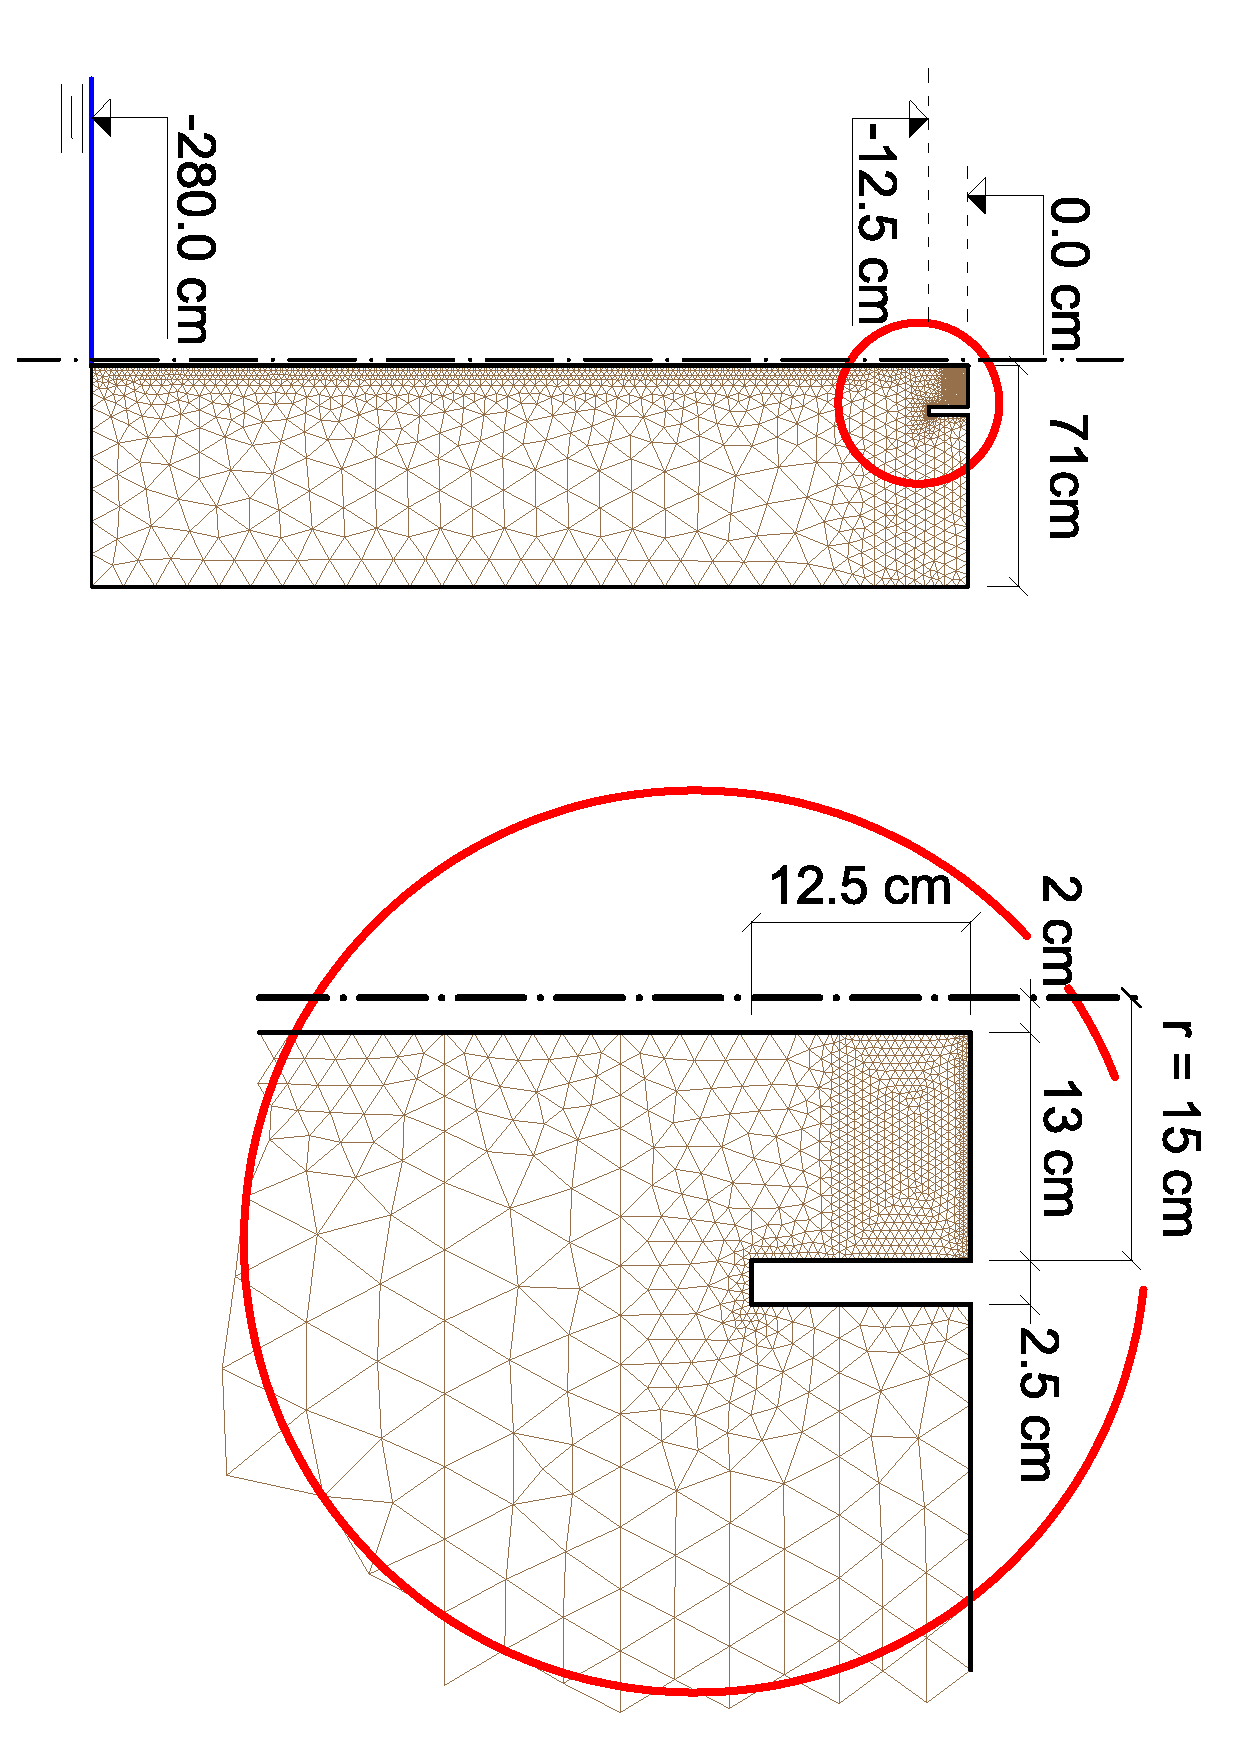
\includegraphics[height=11cm]{infilsit.pdf}}
 \caption{Scheme of the computational domain geometry and domain triangularization.}
 \label{valec}
\end{figure}


%reseni rovnice bylo ve std pojeti, reseni ze sobolevova prostoru funkci definovanych na oblasti z lips hranici
It is well-known that sudden changes in domain shapes, spikes and discontinuities yield numerical difficulties (e.g. the Lipschitz boundary restrictions~\citep{braess}).
In order to avoid computational difficulties during the automatic calibration procedure the infiltration ring thickness was oversized  to 2.5~cm, see figure~\ref{valec}. It is obvious that the real ring thickness is much smaller (in our case 2~mm), but using the real ring thickness yields possible numerical issues. 

\mich{\linelabel{line:thckstart} In order to evaluate the effect of such simplification we have solved the equation~\eqref{richaxi} accompanied with the initial condition~\eqref{icond} and boundary conditions~\eqref{bccond} on domains with the oversized ring thickness of 25~mm and with the real ring thickness of 2~mm. The SHP values were obtained from~\citep{retc} code for clay-loam. The problem was solved on domains with two different mesh discretization setups -- coarse mesh (1013~NDOFs with oversized ring and 1199~NDOFs with real ring thickness) and fine mesh (31848~NDOFs with oversized ring and 32328~NDOFs with real ring thickness).  Details of different domains with different discretizations are depicted in figure~\ref{mesh-eval}. It is apparent that for coarse meshes, the mesh density around the ring edge is governed by the domain shape. In order to validate the results the computation should be done on meshes, where the mesh density is not significantly influenced by the ring shape. Apparently, this is the case of the very fine meshes, where the mesh density $\Delta x$ was equal to the ring thickness (2~mm). The domain triangulation was conducted with T3D mesh generator~\citep{t3d}, which has been successfully used for a number of large scale engineering problems~\citep{rypl2010, kruis2002}. Figure~\ref{mesh-errs} depicts the relation for the difference $I_s(t)-I_r(t)$, where $I_r(t)$ [L] is the cumulative flux across the Dirichlet boundary for the domain representing the real ring thickness, and $I_s(t)$~[L] is the cumulative flux across the Dirichlet boundary on domain representing the oversized ring thickness. It is concluded that with the increased mesh density the difference $I_s(t)-I_r(t)$ vanishes.  And so it becomes apparent, that oversizing the ring thickness does not significantly affect the fluxes through the top Dirichlet boundary, which is the only important part of the solution of~\eqref{richaxi} for our calibration process. \linelabel{line:thckend}

 \begin{figure}
\centering
\rotatebox{90}{
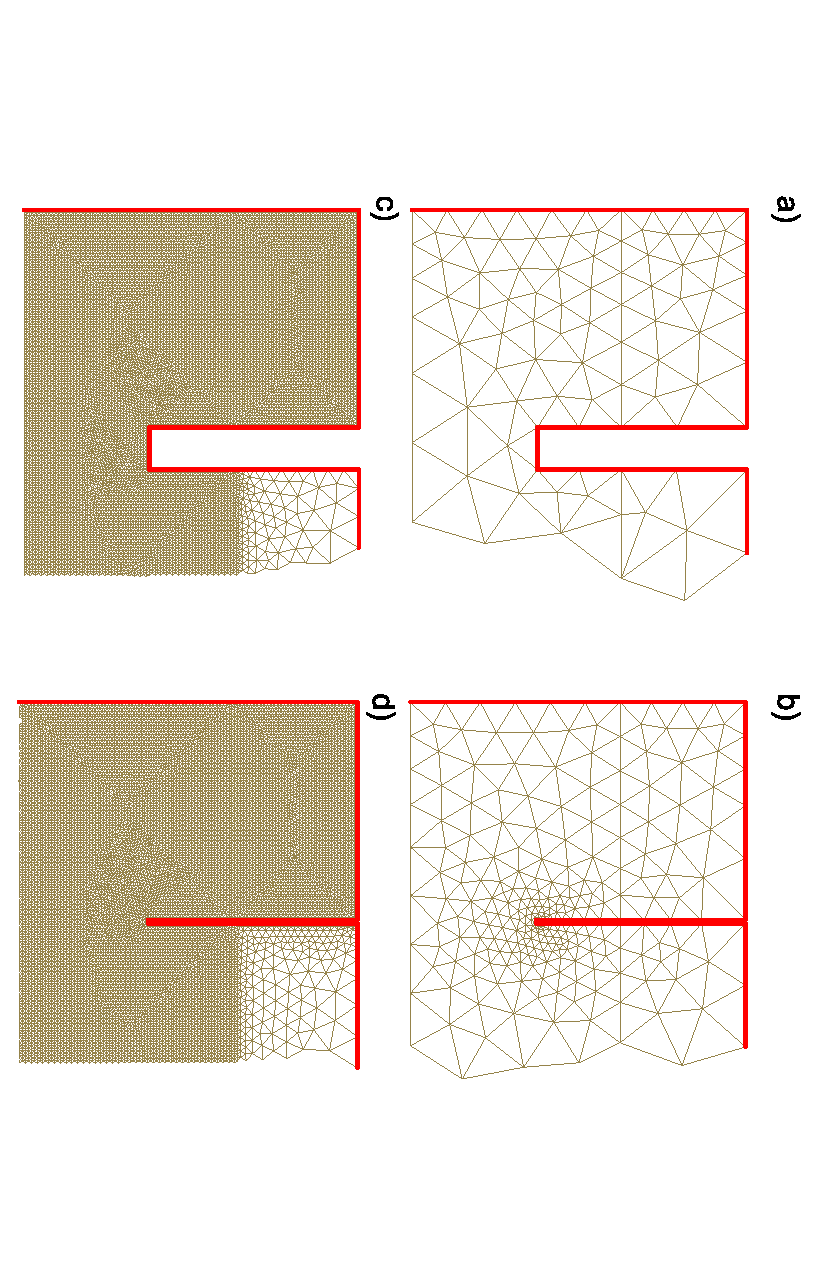
\includegraphics[height=11cm]{data/mesh-evals/site-eval.pdf}}
 \caption{Details of domains with the oversized ring thickness and the real ring thickness discretized with different triangulation densities. Details a) 1013~NDOFs, b) 1199~NDOFs, c) 31848~NDOFs,  d) 32328~NDOFs. }
 \label{mesh-eval}
\end{figure}

 \begin{figure}
\centering
\rotatebox{-90}{
\includegraphics[height=7cm]{data/mesh-evals/meshdiff.eps}}
 \caption{Difference between the cumulative infiltration on domain with real ring thickness $I_r$ and the oversized ring thickness $I_s$. It is apperent, that with the increased mesh density this difference vanishes.}
 \label{mesh-errs}
\end{figure}

}





\subsubsection{Stability restrictions of convection dominant problems}
\label{restrconvect}

The equation \eqref{convect} refers to coefficient  of the first order derivative term in~\eqref{richaxi}, and so the well known stability restrictions for the numerical solutions of the convection-diffusion problems appear here~\citep{zienkiewicz1976}.
The Peclet number representing the numerical stability of convection-diffusion problems is defined as~\citep{knobloch2008} 
\begin{lineq}
\label{peclet-std}
Pe = \frac{c \Delta x}{2 D},
\end{lineq}
where $c$ is the convection coefficient defined in~\eqref{convect}, $\Delta x$ is the discretization step, and $D$ is the diffusion (for isotropic setup). Based on the definitions given above, equation~\eqref{peclet-std} can be formulated as
\begin{lineq}
\label{peclet-re}
Pe =  \frac{\frac{1}{r}K(h) \Delta x}{2K(h)} = \frac{\Delta x}{2r}.
\end{lineq}
Since our mesh is triangular, $\Delta x$ can be roughly assumed to be the greatest triangle altitude (since we assume some mesh quality properties). Then a sufficient distance from the axis of axisymmetry is such that the Peclet number is sufficiently low. If we want to make our computation free of the well
  known spurious oscillations~\citep{zienkiewicz1976, roos-layers}, 
a sufficiently low Peclet number $Pe\le 1$ is required. Therefore, the distance from the axis of axisymmetry is given by the domain discretization step at 
the left hand side boundary. The selected discretization step at the left hand side boundary was assumed as $\Delta x=2$~cm. The domain was therefore 
detached by 2~cm from the axis of axisymmetry, and thus the Peclet number was 0.5 only. \mich{\linelabel{line:convstart} This simplification must be again validated. However, compared 
to the oversized ring thickness, it is impossible to numerical model domains, where $r_{min}=0$ (where $r_{min}$ is the minimum distance of the domain from the center of axisymmetry).  And so three different setups, where the domain was 
detached for $r_{min}=$~0.2,~1.0, and 2.0~cm from the center of axisymmetry, were tested. In order to maintain the Peclet number on equal level, the mesh density
 $\Delta x$ at the left hand side boundary should be equal to $r_{min}$. It is apparent, that compared to the previous case, where we were evaluating the oversized ring thickness, changing the location of the left hand side boundary will significantly affect the mesh size, as depicted in figure~\ref{mesh-dens}. In order to obtain comparable data,  three different domains with $r_{min}=0.2$,~1.0, and 2.0~cm  were triangularized with equal mesh densities given by the lowest $r_{min}$  (in order to obtain comparable data). It turns out, that for $r_{min}=2.0$~cm the Peclet number~\eqref{peclet-re} was $Pe=0.05$, and the mesh size was 10851~NDOFs, for $r_{min}=1.0$~cm the Peclect number was $Pe=0.25$, and the mesh size was 100036~NDOFs , and for $r_{min}=0.2$~cm the Peclet number was $Pe=0.5$, and the mesh size was 10156~NDOFs. Since the Peclet numbers are already very low, the solutions are free of spurious oscillations, and can be compared. Please note, that the mesh sizes with decreasing $r_{min}$ doesn't increase monotonously, since the mesh is non-uniform and different mesh density and domain shape configurations lead to different triangularizations.
 
 Similarly to the previous section~\ref{shaperestr}, the equation~\eqref{richaxi} accompanied with the initial~\eqref{icond} and boundary conditions~\eqref{bccond} was solved on three different domains with $r_{min}=0.2$,~1.0,~2.0~cm. The SHP values were again obtained from~\citep{retc} code for clay-loam. The figure~\ref{mesh-evals2} depicts the difference between the cumulative volumetric flux across  the top Dirichlet boundary for the domains with $r_{min}$ offset 2.0~cm and 1.0~cm, and with $r_{min}$ offset 2.0~cm and 0.2~cm. It is apparent, that while decreasing the offset with ratios 0.5 and 0.1 the differences between the cumulative fluxes maintain similar order of magnitude. The differences probably originate from different domains triangularizations, and are below the data resolution originating from in-situ experimental conditions. \linelabel{line:convend}
 
 }



 \begin{figure}
\centering
\rotatebox{-90}{
\includegraphics[height=7cm]{data/mesh-dens/denses.eps}}
 \caption{Relation between the distance from the axis of axisymmetry ($r_{min}$) and the mesh size (NDOFs), while maintaining the Peclet number of convective dominance~\eqref{peclet-re} at constant level. Over 100 meshes with T3D mesh generator~\citep{t3d} were generated for this plot, the relation is not monotoneous, since different mesh densities yield different triangularizations.}
 \label{mesh-dens}
\end{figure}


 \begin{figure}
\centering
\rotatebox{-90}{
\includegraphics[height=7cm]{data/mesh-evals2/mesh-diff.eps}}
 \caption{Difference between the cumulative volumetric flux across  the top Dirichlet boundary for the domains with $r_{min}$ offset 2.0~cm and 1.0~cm, and with $r_{min}$ offset 2.0~cm and 0.2~cm.}
 \label{mesh-evals2}
\end{figure}



\subsection{Optimization}

\subsubsection{Objective function} %[michal]
\label{objdef}

\mich{In this section the methodology for identification of the SHP parameters from the Richards equation will be presented.}
Since the parameters will be identified using a stochastic method \mich{and gradient method with constraints, we have to introduce a  range for each parameter. The ranges for the SHP for the intial parametric space search are specified in table~\ref{rozsahy}, the ranges for the gradient method with contraints will be specified later.} These initial ranges are very broad, since we are trying to explore a possible non-uniqnuess of this inverse model \mich{even beyond physically acceptable ranges}.

\begin{table*}[ht]
\begin{center}
\caption{Ranges of SHP ($\vec{p}_{max}$ and $\vec{p}_{min}$) for identifying the SHP in the top-soil layer for {\it refinement level} $r_f=0$. Note that the initial ranges are extremely broad especially for the saturated water content $\theta_s$. This broad range was selected in order to explore the uniqnuess
of the REVG inverse model of SR experiment
 even beyond the physically acceptable solutions. }
\fs
\begin{tabular}{c | c| c| c| c}
\toprule
% Ranges of depths, horizon(s)&\multicolumn{4}{c}{Input values for inverse modelling}\\ \cline{2-5}
$\theta_s$ [-]&$\alpha$ [cm$^{-1}$]&n [-]& $K_s$ [cm.hrs$^{-1}$] & $S_s$ [cm$^{-1}$] \\ \hline
\toprule
0.25 -- 0.90 & \num{0.01e-2} -- \num{5.0e-2} & 1.05 -- 4.5 & 0.300 -- 300.0 & 0.0 -- 0.1 \\
\toprule
\end{tabular}
\label{rozsahy}
\end{center}
\end{table*}

The objective function is defined in the following paragraph.


Let $\bar{I}(\vec{p},t)$ be the cumulative infiltration obtained from solving the mathematical model~\eqref{richaxi} bounded by the initial and boundary conditions  defined in section~\ref{bccond} for a certain vector of SHP parameters $\vec{p}$ considered as
\begin{lineq}\bar{I}(\vec{p},t) = \frac{\int\limits_0^t \int\limits_{\Gamma_1}-K \frac{\partial H}{\partial \vec{n}}(t)  \dd \Gamma_1 \dd t}{\int\limits_{\Gamma_1} \dd \Gamma_1}.\end{lineq}
Let $I(t)$ be the cumulative infiltration given by \eqref{vyhlaz} with parameters given in section~\ref{site}.  
Then the objective function was defined for three different criteria in order to avoid ill-posed objective function definition.

 Both $\bar{I}(\vec{p},t)$ and $I(t)$ are continuous functions. Note please, that this is not a standard configuration. The objective functions were then defined as follows:
\begin{enumerate}[label={\bf \Roman*}.]
\item First criterion $\Psi_1$ was defined as $\mathcal{L}_2$ norm of the difference between the  experimental and model data and thus
\begin{lineq}
\label{objektiva1}
\Psi_1 (\vec{p}) = \frac{\sqrt{\int\limits_0^{T_{end}} \left( \bar{I}(\vec{p},t) - I(t) \right)^2 \dd t}}{T_{end}},
\end{lineq}
where $T_{end}$ is the final simulation time [$T$], which is indeed the root mean square error (RMSE) for continuous functions. 
\item Second criterion was the $\mathcal{L}_{\infty}$ norm of the difference between the experimental and model data and thus
\begin{lineq}
\label{objektiva2}
\Psi_2 (\vec{p}) = \mathrm{sup} \left( \sqrt{\left( \bar{I}(\vec{p},t) - I(t) \right)^2} \right), \quad  t \in (0, T_{end}).
\end{lineq}
\item Third criterion was considered as the difference between the infiltration rates (final derivatives) between the model data and the experimental data
\begin{lineq}
\label{objektiva3}
\Psi_3 (\vec{p}) =  \sqrt{\left( \frac{\dd \bar{I}(\vec{p},T_{end})}{\dd t} - \frac{\dd I(T_{end})}{\dd t} \right)^2}.
\end{lineq}


\end{enumerate}

\mich{\linelabel{line:objstart} The first objective function~\eqref{objektiva1} refers to overall mismatch between the experimental and model data. The second objective function~\eqref{objektiva2} refers to a local mismatch, which  often appeared  in the early simulation time. Slight local mismatch in the initial simulation has typically low impact on~\eqref{objektiva1}, but points to a significantly different SHP set -- a local extreme. The strategy, where we focus both on the global and local error is motivated by~\cite{papez2014}, where it states that the reliable stopping criteria for iterative algebraic solvers should  take into account spatial distribution of the total error in the function space.
The third objective function~\eqref{objektiva3} points to saturated hydraulic conductivity. Again slight mismatch in the final derivatives has low impact on the first objective function~\eqref{objektiva1}, but points to a significantly different saturated hydraulic conductivity.\linelabel{line:objend} }

\linelabel{line:multistart} We conducted multi-objective optimization. However, it is apparent that minimizing the objective function~\eqref{objektiva1} also minimizes the objective functions~\eqref{objektiva2} and \eqref{objektiva3}, \mich{and so we have introduced here a multiobjective definition with  non-competing objective functions. 

The major benefit of multi-objective optimization  to solve typically single objective inverse problems is to speed-up the convergence in
case of non-competing objective functions.

This multi-objective approach  for parameter estimation is inspired by \cite{knowles:2001} where the authors expand the
single-objective problem to the multi-objective space by replacing the original objective with a~set of new objectives
or new objectives are added to the original one. The idea is to give an~algorithm more freedom to explore the search
space and, therefore, decreases the probability to be trapped in a~local extreme. Although superfluous at the first
view, in many cases the speed-up to the original single-objective optima was higher in the multi-objective case.
Similar idea is behind {\it helper} objectives~\citep{Jensen:2004}, however, the computational advantage of the
multi-objective application is problem-dependent, see \citep{vitingerova:2010} and references therein.



Many classical material models have independent sets of parameters for different phenomena and thus the error
functions are non-competing. However, in many models, especially phenomenological ones, some parameters influence
several model's outputs and therefore, they are dependent and the objectives can be competing.

It must be pointed out that the perfect fit should not exist for real data because of the 
model approximation errors, errors in model numerical representation, and 
measurements errors (note please that measurement errors were not evaluated here). Thus the individual error
functions can be minimized towards the zero individually but not jointly.
Similar applications can be found in papers by  \cite{Kuraz:2010:JCAM} or \cite{Gong:2015}. \linelabel{line:multiend}





}






\subsubsection{Optimization algorithms}%[matej]
\label{optima}

\paragraph{Genetic algorithm}

In this contribution we used the modified genetic algorithm GRADE \citep{grade,Kucerova:2007:PHD} supported by niching method CERAF~\citep{Hrstka} enhancing the algorithm with
memory and restarts. \mich{\linelabel{line:gradestart} GRADE is a real-coded genetic algorithm combining the ideas of genetic operators: cross-over, mutation and selection
taken from the standard genetic algorithm and differential operators taken from differential evolution. In more detail,
a new population is created with the same size as the old population by 40\% using a vectorized mutation and 60\% by
the differential cross-over, see references above for particular details. Then the next generation is created by
survival selection employing an inverse tournament selection, where the worse from two competitors is rejected
repeatedly until the original size of the population is reached. In our case, the population of the genetic
algorithm contains 30 independent solutions, 12 new solutions are created by mutation and 18 by cross-over, respectively. The whole identification stops after 40.000 evaluations of the problem \linelabel{line:gradeend} simulations.

When GRADE algorithm converges, the current position of the optimization algorithm is marked as a local extreme, is
stored in a memory, and a forbidden area is built around it in order to avoid the optimization algorithm to fall into
the same local extreme again and the whole algorithm is re-started. In our case a~local extreme was marked after 600
evaluations without any improvement.}

GRADE project is capable for multi-objective definition for the objective function, which is achieved with so-called
 Average Ranking (AR) \citep{Leps2007}. It sums ranks of the objective functions instead of the objective functions' values. Therefore, no weights are needed, however, the Pareto non-dominance is not preserved as described in \cite{vitingerova:2010}. An application of the AR algorithm to parameters identification can be found in \cite{Kuraz:2010:JCAM}. 

 
 
 \mich{
 \paragraph{Gradient algorithm} 
 
 Since achieving a fully converged solution with genetic algorithms can be cumbersome, as well as the selected optimal position at the Pareto front from the multi-objective minimization doesn't necessarily point to the  local minimum of each objective function, the following strategy was considered here. The genetic algorithm was used here as an estimator of the initial condition for further gradient parameter search on narrow ranges. For gradient optimization we made use of Newton's method with box-constraints~\citep{byrd1995}, implemented in R environment~\citep{R-env}. Compared to the genetic algorithm optimization, only single objective criteria given by~\eqref{objektiva1} is minimized here.
}


\subsection{Numerical solution and computational issues}
\label{trapoty}

Equation~\eqref{richaxi} was implemented into the DRUtES library~\citep{drutes}. It is an object-oriented library written in Fortran 2003/2008 standard for solving nonlinear coupled convection-diffusion-reaction type problems. The problem was approximated by the linear finite element method for spatial derivatives and Rothe's method for temporal derivatives. The nonlinear operator was treated with the Schwarz-Picard method -- an adaptive domain decomposition  ($dd$-adaptivity) -- with the ability to activate and deactivate subregions of the computational domain sequentially ~\citep{mojecomp, mojejcam2, mojeamc2}.



 The domain was non-uniformly discretized by a triangular mesh. The smallest spatial step was considered for the top layers inside the infiltration ring, close to the Dirichlet boundary. The mesh is depicted in figure~\ref{valec}. The minimum spatial length was 0.5~cm, and the maximum spatial length was 20~cm. The domain was discretized with 2097 nodes and 3861 elements. The coarse mesh for the $dd$-adaptivity method was a uniform quadrilateral mesh with elements 17.75$\times$28.0~cm, i.e. a total of 40 coarse elements and 55 nodes. The purpose of the coarse mesh is to organize the elements of the domain triangularization into so-called clusters, which form a basic unit for the adaptive domain decomposition used here for solving the nonlinear problem, details can be found in~\citep{mojeamc2}.

 
 The spatial and temporal discretization of \eqref{richaxi} leads to sequential solutions of systems of non-linear equations, see e.g.~\citep{mojecomp}. The system was linearized as discussed in~\citet{mojeacta, mojeamc}, and so the numerical solution requires an iterative solution of 
\begin{lineq}
\label{matice}
\mathbf{A}(\vec{x}_l^k) \vec{x}_l^{k+1} = \vec{b}(\vec{x}_l^k),
\end{lineq}
where $k$ denotes the iteration level, and $l$ denotes the time level, until \begin{lineq} \label{picard} ||\vec{x}_l^{k+1} - \vec{x}_l^k||_2 < \varepsilon , \end{lineq} where $\varepsilon$ is the desired iteration criterion.  It is apparent that the number of required  iterations depends on the $\varepsilon$ criterion. 


The method~\eqref{matice} degenerates into a kind of semiexplicit approximation if the error criterion $\varepsilon$ was "infinitely huge" (it means taken from the extended real numbers, $\varepsilon \in {\overline {\mathbb {R} }}$, and assigned as $\varepsilon = + \infty$). This semiexplicit approximation is denoted as
\begin{lineq}
\label{matice2}
\mathbf{A}(\vec{x}_{l-1}) \vec{x}_l = \vec{b}(\vec{x}_{l-1}).
\end{lineq}
 This semiexplicit method always requires just a single  iteration. With a short time step the method converges to the exact solution. For inappropriate time steps, the method diverges from the exact solution faster than the method~\eqref{matice}. Nonetheless, the method~\eqref{matice2} is free of possible issues related to the convergence of the nonlinear operator.



\section{Automatic calibration methodology}%[michal]
\label{methodo}



%It was taken into consideration that the available experimental input data refers to cumulative infiltration flux. The infiltration flux is obtained from the numerical derivative of the solution of \eqref{richaxi}. 
We address possible difficulties with convergence of the linearized discrete system~\eqref{matice} for certain combinations of SHP parameters during the automatic calibration, as discussed by~\cite{beven2003-uncertain}.
Moreover, we address the problem of multimodality when the initial range of SHP parameter is broad as in table~\ref{rozsahy}.
It is known that inaccurate approximation of the capacity term (time derivative term) yields inaccurate mass properties~\citep{celia} and are aware of the possible impact of spatial and temporal discretization on the identified SHP values.  

Following the concerns about effects of the numerical treatment on the identified SHP, we propose an automatic calibration methodology depicted in figure~\ref{flowchart}. Details are given in the following algorithm scheme. In brief, the proposed method uses less accurate, but fast and convergence-issue-free numerical technique, to identify (several) promising parameter regions. To avoid the influence of the numerical solver setup,  the SHP estimate is consequently updated in each parameter region with an improved numerical treatment of the Richards equation solver. It is presumed that the inverse model solution is non-unique on the initial broad parameter range, but unimodal on the narrow region(s), which are subsequently investigated. 

Let us define the following nomenclature: % I really wanted to say here Let us define :) I think it's fine here :)

\hrulefill
\begin{description}
\item[$r_f$] -- "refinement level", the problem is treated with different spatial and temporal discretization setups, each setup is denoted by value of $r_f$ index,
\item[$i_e$] -- local extreme index,
\item[$\vec{p}$] -- vector of SHP parameters, vector contains the values of $\alpha$, $n$, $\theta_s$, $K_s$, $S_s$,
\item[$\vec{p}_{max,min}^{r_f}$] -- maximal, resp. minimal values of SHP parameters defining a parameter range for a certain refinement level $r_f$,
\item[$\vec{p}_{max,min}^{ i_e, r_f}$] -- maximal, resp. minimal values of SHP parameters defining a parameter range for a certain refinement level $r_f$ in a certain vicinity of a local extreme $i_e$,
\item[$\Delta(\vec{x})$] -- spatial discretization (mesh density, mesh is non-uniform).
\end{description}
\hrulefill


\begin{figure*}
\centering
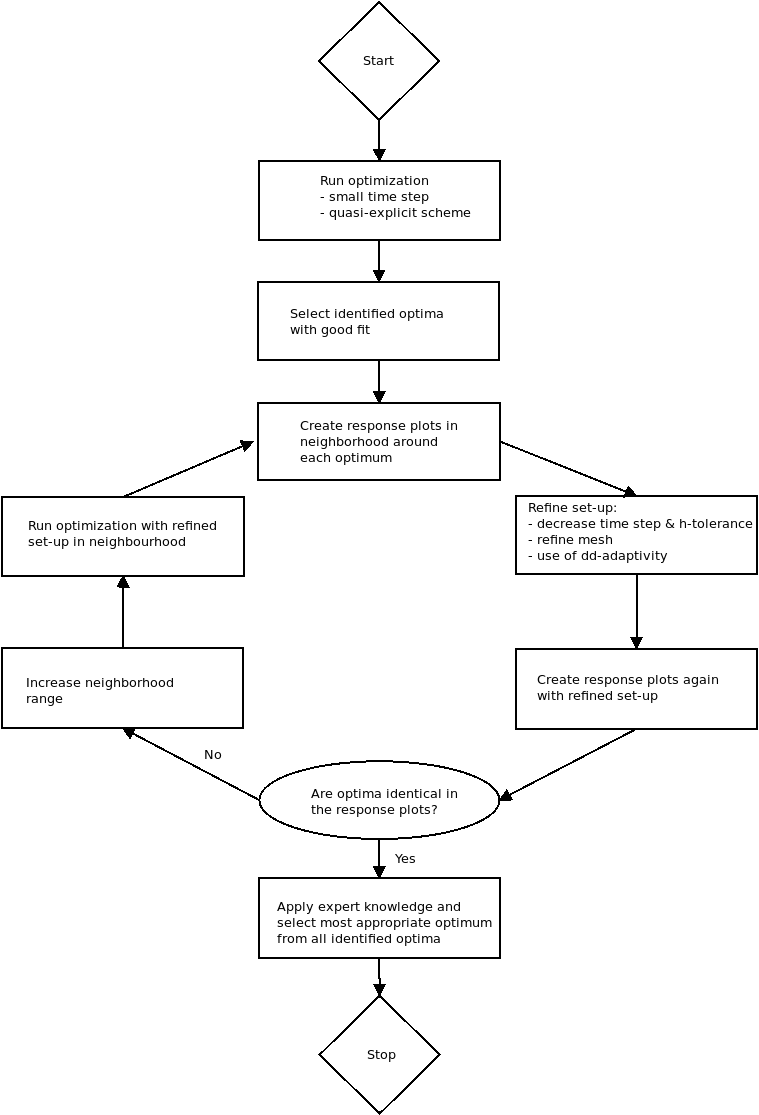
\includegraphics[width=12cm]{flowchart/Flow_chart_cb_new.png}
\caption{The proposed methodology for the automatic calibration avoiding effects of numerical treatment for the identified SHP values.}
\label{flowchart}
\end{figure*}

The calibration algorithm is described as follows:

 \begin{enumerate}[label={\bf [\Roman*.]}]
    \item  {\bf Do} initial calibration  with genetic algorithm GRADE~\citep{grade} and with semiexplicit method~\eqref{matice2} ($\varepsilon \leadsto +\infty$), $r_f$=0,  vectors $\vec{p}_{max,min}^{r_f}$ are taken from table~\ref{rozsahy}
     \item \label{docal} {\bf Create}  sequence of vectors $\vec{\bar{p}}^{i_e}_{r_f}$.\mich{ Please note that these extremes are typically parameter sets in a vicinity of a minimum of the objective function~\eqref{objektiva1}.}
         \begin{itemize} \item {\bf If} the problem is multimodal 
       \begin{itemize} 
           \item {\bf then} $i_e > $ 1, 
           \item {\bf else} $i_e = $ 1.
       \end{itemize} 
       \end{itemize}
      \item \label{gradient} \mich{{\bf For each } vector  $\vec{\bar{p}}^{i_e}_{r_f}$ conduct gradient optimization using {\bf single} objective~\eqref{objektiva1} with Newton's method with box-constraints~\citep{byrd1995} on parameter ranges $\vec{p}^{i_e, r_f}_{max} = 1.1\vec{\bar{p}}^{i_e}_{r_f}$ and $\vec{p}^{i_e, r_f}_{min} = 0.9\vec{\bar{p}}^{i_e}_{r_f}$, where the initial estimate is obtained from the genetic algorithm solution $\vec{\bar{p}}^{i_e}_{r_f}$, so that the converged solution $\vec{p}^{i_e}_{r_f}$ is ensured. }

 \item \label{validation} {\bf Do validation:}  
    \begin{enumerate} 
      \item {\bf select} local extremes with good fitting qualities,
        \item {\bf increase} $r_f=r_f+1$ as follows 
                  \begin{lineq}
                  \label{coeffs}
                  \begin{split}
                  \Delta(\vec{x})^{r_f}  &= \frac{\Delta(\vec{x})^{r_f-1}}{2}, \\
                  \varepsilon^{r_f} &= 10^{-3} \; \mbox{cm} \quad  \mbox{if} \; r_f = 1, \; \; \\ &\mbox{else} \quad \varepsilon^{r_f} = \frac{\varepsilon^{r_f-1}}{10}, \\
                  t_{init}^{r_f} &=  \frac{t_{init}^{r_f-1}}{10} \; \mbox{hrs} .
                  \end{split}
                  \end{lineq}
        \item {\bf create} a response plot of \eqref{objektiva1} for current $r_f$ and $r_f-1$ in the neighborhood defined as 
            \begin{lineq}
            \label{parrange}
              \begin{split}
              \vec{p}^{i_e, r_f}_{max} &= 1.25\vec{p}^{i_e}, \\
              \vec{p}^{i_e,r_f}_{min} &= 0.75\vec{p}^{i_e}. 
              \end{split}
            \end{lineq}
            
       \item {\bf Validation methodology:}
       
       \begin{enumerate}
       \item Visually {\bf inspect} response  plots for the selected local extreme $i_e$ created with discretization $r_f$ and $r_f-1$.
       \item \label{cond} {\bf If} the response plots differ significantly,
       \begin{itemize}
          \item \mich{ {\bf then} {\bf redefine} the parameter range as specified in~\eqref{parrange}, {\bf return} to \ref{gradient},
          start a {\bf gradient optimization}, where the initial estimate is $\vec{p}_{r_f-1}^{i_e}$. {\bf For each} local extreme $i_e$
            new sets of vectors  $\vec{p}_{r_f}^{i_e}$ will be generated, {\bf go to}  \ref{validation} and {\bf proceed new validation}. } 
          \item {\bf else} {\bf exit} the calibration process.
      \end{itemize}
\end{enumerate}

\end{enumerate}
\end{enumerate}

\mich{\linelabel{line:expstart} At the end of this calibration process we typically finish with a set of solutions $\vec{p}^{i_e}$, where $i_e \in \{1, ..., \mbox{[number of extremes]} \}$. At this stage the {\it expert knowledge} should be incorporated as a final decision making mechanism for obtaining the unique solution.  Despite the exact value of $\theta_s$ is not necessarily known, and so it can't be removed from the searched parametric space, acceptable ranges of $\theta_s$ form a part of the expert knowledge. The appropriate parametric set will be selected from the list of identified solutions on the basis of expected values of $\theta_s$ parameter. \linelabel{line:expend}} 

\mich{
\subsection{Mathematical model of the synthetic infiltration experiment}

The purpose of this benchmark example was to demonstrate, whether this class of problem -- identification of SHP parameters from cumulative flux measured at Dirichlet boundary -- can be affected by multimodality.


 For simplicity only a one-dimensional infiltration problem was considered here. The governing equation~\eqref{richaxi} can be now formulated for one-dimensional problem as follows
 \begin{lineq}
 \frac{\dd \theta}{\dd h}\frac{\partial h}{\partial t} = \frac{\partial K(h) \frac{\partial  H}{\partial z}}{\partial z}.
 \end{lineq}

 
 
 
 
 Dirichlet boundary conditions were presumed for both boundaries. The model setup state as follows. Computational domain was $\Omega=(0,100\,\mathrm{cm})$, and the boundary and initial conditions stated as follows
 \begin{lineq}
 \begin{split}
 h(z,t) &= 0\, cm, \quad \forall (z,t) \in \Gamma_{bot} \times  t \in [0, T_{end}) \\ 
  h(z,t) &= 0\, cm, \quad \forall (z,t) \in \Gamma_{top} \times  t \in [0, T_{end}) \\ 
  H(z,t_0) &= 0\, cm , \quad \forall z \in \Omega,
  \end{split}
\end{lineq}
 where $\Gamma_{bot}=0.0$ cm, $\Gamma_{top}=100.0$ cm, and $T_{end}=$\num{e-1}~hrs. Two distinguished soil types were considered here -- clay loam and sand, the parameters were obtained from~\citep{retc}.
 

 
  The computational domain $\Omega$ was uniformly discretized with $\Delta x$=0.5~cm, the initial time step was $\Delta t$=\num{e-7}~hrs, and the error criterion from~\eqref{picard} for solving the nonlinear system~\eqref{matice} was   $\varepsilon$=\num{e-3}~cm.
 
 The reference solutions both for sand and gravel media were obtained from  cumulative flux over the top Dirichlet boundary $\Gamma_{top}$.
 
For the given reference solutions the genetic algorithm described in section~\ref{optima} was employed for searching the original SHP parameters in broad ranges given in table~\ref{rozsahy}. 
In order to avoid effects of numerical treatment of the Richards equation, the numerical solver had exactly the same configuration as the one used for the reference solution.



}


 



\section{Results and discussion} 

This section begins with a simple synthetic problem with known exact solution, which is given here to test the possible multimodality of the conducted inverse modeling of infiltration experiment, to provide a support for the methodology given in section~\ref{methodo}. Later,  we continue in section~\ref{rworld} with presenting our real world problem example, where we  present our parameter estimate for the top soil organic horizon, obtained from the methodological approach explained above in~\ref{methodo}.

\subsection{Synthetic problem}
 \label{benchmarks}
 
 
 
Results of the synthetic problem are given in table~\ref{tab-benchres}. For these two different soil types involved  the inverse modeling algorithm has found several local optima, and the low value of an objective function doesn't necessarily  point to the correct solution. Thus the problem is multi-modal. Several distinct SHP parameter sets can lead to acceptable solutions. However, the most distinct SHP parameter is the saturated water content $\theta_s$. \mich{It turns out that approximate knowledge of $\theta_s$ -- the expert knowledge --- is required to select an acceptable solution of this inverse problem. }\mich{ The results of this synthetic problem supports the methodology given in section~\ref{methodo}.}



\begin{table*}[]
\centering
\caption{Results of the synthetic problem. The grey highlighted rows refer to the physically acceptable solution of this benchmark inverse problem, and the red highlighted rows contain the exact solution of this inverse problem.}
\label{tab-benchres}
\footnotesize
\begin{tabular}{|c|c|c|c|c|c|c|c|}
\hline
\multicolumn{3}{|c|}{\cellcolor[HTML]{34CDF9}}                                                                                                                        & \multicolumn{4}{c|}{parameters}                                                                                                                                                                                                                            &                                             \\ \cline{4-7}
\multicolumn{3}{|c|}{\multirow{-2}{*}{\cellcolor[HTML]{34CDF9}}}                                                                                                      & $\alpha$ [cm$^{-1}$]                                          & $n$ [-]                                                      & $\theta_s$ [-]                                               & $K_s$ [cm.hrs$^{-1}$]                                        & \multirow{-2}{*}{RMSE error}                \\ \hline
                                     & \multicolumn{2}{c|}{\cellcolor[HTML]{CB0000}{\color[HTML]{FFFFFF} \textbf{exact solution}}}                                    & \cellcolor[HTML]{CB0000}{\color[HTML]{FFFFFF} \textbf{0.019}} & \cellcolor[HTML]{CB0000}{\color[HTML]{FFFFFF} \textbf{1.31}} & \cellcolor[HTML]{CB0000}{\color[HTML]{FFFFFF} \textbf{0.41}} & \cellcolor[HTML]{CB0000}{\color[HTML]{FFFFFF} \textbf{6.24}} & \cellcolor[HTML]{34CDF9}                    \\ \cline{2-8} 
                                     &                                                                                           & \cellcolor[HTML]{C0C0C0}\textbf{1} & \cellcolor[HTML]{C0C0C0}0.020                                 & \cellcolor[HTML]{C0C0C0}1.321                                & \cellcolor[HTML]{C0C0C0}0.395                                & \cellcolor[HTML]{C0C0C0}6.226                                & \cellcolor[HTML]{C0C0C0}\num{0.04787}       \\ \cline{3-8} 
                                     &                                                                                           & \textbf{2}                         & 0.012                                                         & 1.050                                                        & 0.250                                                        & 7.011                                                        & \num{0.2830367232}                          \\ \cline{3-8} 
\multirow{-4}{*}{\textbf{clay loam}} & \multirow{-3}{*}{\textbf{\begin{tabular}[c]{@{}c@{}}identified\\ solutions\end{tabular}}} & \textbf{3}                         & \num{0.00012796}                                              & 1.146                                                        & 0.900                                                        & 94.904                                                       & \num{0.3724314113}                          \\ \hline
\multicolumn{8}{|l|}{\cellcolor[HTML]{656565}}                                                                                                                                                                                                                                                                                                                                                                                                                                   \\ \hline
                                     & \multicolumn{2}{c|}{\cellcolor[HTML]{CB0000}{\color[HTML]{FFFFFF} \textbf{exact solution}}}                                    & \cellcolor[HTML]{CB0000}{\color[HTML]{FFFFFF} \textbf{0.145}} & \cellcolor[HTML]{CB0000}{\color[HTML]{FFFFFF} \textbf{2.68}} & \cellcolor[HTML]{CB0000}{\color[HTML]{FFFFFF} \textbf{0.43}} & \cellcolor[HTML]{CB0000}{\color[HTML]{FFFFFF} \textbf{29.7}} & \cellcolor[HTML]{34CDF9}                    \\ \cline{2-8} 
                                     &                                                                                           & \textbf{1}                         & 0.039                                                         & 1.050                                                        & 0.250                                                        & 35.563                                                       & \num{0.02977800386}                         \\ \cline{3-8} 
                                     &                                                                                           & \textbf{2}                         & 0.026                                                         & 1.087                                                        & 0.587                                                        & 37.877                                                       & \num{0.02405719725}                         \\ \cline{3-8} 
\multirow{-4}{*}{\textbf{sand}}      & \multirow{-3}{*}{\textbf{\begin{tabular}[c]{@{}c@{}}identified\\ solutions\end{tabular}}} & \cellcolor[HTML]{C0C0C0}\textbf{3} & \cellcolor[HTML]{C0C0C0}0.154                                 & \cellcolor[HTML]{C0C0C0}2.654                                & \cellcolor[HTML]{C0C0C0}0.460                                & \cellcolor[HTML]{C0C0C0}30.145                               & \cellcolor[HTML]{C0C0C0}\num{0.02198515637} \\ \hline
\end{tabular}
\end{table*}






% clay with original settings
%  0.020367, 1.3219, 0.39551, 6.2261  0.04787
% 0.011519, 1.05, 0.2502, 7.0108 0.2830367232
%  0.00012796, 1.1462, 0.9, 94.904 0.3724314113
 
%  clay with semi-explicit
% 0.019941, 1.3504, 0.46568, 7.005 0.560637688
%  0.094183, 3.7989, 0.25003, 3.8626 1.290496494
% 0.019983, 1.35, 0.26555, 6.9927 0.6542315846

% sand with original settings
% 0.039412, 1.0502, 0.25018, 35.563 0.02977800386
% 0.026293, 1.0872, 0.58662, 37.877 0.02405719725
% 0.154 & 2.6543 &  0.46 & 30.145 0.02198515637 

%sand with semiexplicit
%  0.042468, 1.1269, 0.25569, 69.785 0.0157830282
% 0.12224    2.45494       0.35    32.6334 0.0139951908


\subsection{Real-world problem}
\label{rworld}

 We found multiple optima for the real-world problem. The local extremes for the refinement level $r_f=0$ are given in table~\ref{shp-vysledky}, where the gray lines refer to local extremes with bad fitting properties (extremes 1-5), the local extremes 6-8 refer to inverse model solutions with good fitting properties. The results were visually inspected. An example of bad fitting dataset is depicted in figure~\ref{rf0samples} - left, and the example of the good fitting dataset is depicted in figure~\ref{rf0samples} - right. Solution for each dataset is  given in Appendix. Complete settings specifications for each $r_f$ level involved here are given in table~\ref{tab:rfset}.







% 
% \begin{table*}
% \begin{center}
% \caption{Identified local extremes of Pareto front during the first run of parameter search procedure.}
% \fs
% \begin{tabular}{l || c c c c c  }
% \toprule
% no. & $\alpha$ [cm$^{-1}$] & $n$ [-] & $\theta_s$ [-] & $K_s$ [cm.hrs$^{-1}$] & $S_s$  [cm$^{-1}$] \\ \hline \hline
% \rowcolor{gray}{\bf 1} & \num{2.447e-4} &  2.45 & 0.25 & \num{0.025} & \num{0.419e-2}   \\ 
% \rowcolor{gray}{\bf 2} & \num{0.101e-2} & 0.6517 &  0.271 & \num{1.092} &  \num{2.879e-2}  \\ 
% \rowcolor{gray}{\bf 3} & \num{1.840e-2} & 2.098 & 0.353 & \num{1.092} & \num{1.845e-4} \\
% \rowcolor{gray}{\bf 4} & \num{0.157e-2} & 1.968 & 0.720 & \num{2.07} & \num{1.053e-5}  \\ 
% \rowcolor{gray}{\bf 5} & \num{0.150e-2} & 1.586 & 0.720 &  \num{1.093} &  \num{7.641e-3}  \\ \hline \hline
% \rowcolor{white}{\bf 6} & \num{0.258e-2} & 2.152  & 0.401 &  \num{1.095} & 0  \\ 
% \rowcolor{white}{\bf 7} & \num{0.3802e-2} & 1.279 & 0.594 &  \num{1.165} & 0  \\ 
% \rowcolor{white} {\bf 8} & \num{0.255e-2} & 1.384 & 0.254 &  \num{1.119} &  \num{1.922e-4}  \\ \hline
% \toprule
% \end{tabular}
%  \label{shp-vysledky}
% \end{center}
% \end{table*}


% Please add the following required packages to your document preamble:
% \usepackage{multirow}
\begin{table*}[]
\begin{center}
 \caption{Identified local extremes of Pareto front during the first run of parameter search procedure.}
 \fs
\begin{tabular}{|c||c|c|c|c|c||c|c|}
\hline
                         &                                        &                           &                                  &                                         &                                      & \multicolumn{2}{c|}{RMSE error \eqref{objektiva1} [cm]}                                                              \\ \cline{7-8} 
\multirow{-2}{*}{no.}    & \multirow{-2}{*}{$\alpha$ [cm$^{-1}$]} & \multirow{-2}{*}{$n$ [-]} & \multirow{-2}{*}{$\theta_s$ [-]} & \multirow{-2}{*}{$K_s$ [cm.hrs$^{-1}$]} & \multirow{-2}{*}{$S_s$  [cm$^{-1}$]} & $r_f$ =0          & $r_f$ = 1                                                                                        \\ \hline \hline
\rowcolor[HTML]{C0C0C0} 
{\bf 1}                  & \num{2.447e-4}                         & 2.450                     & 0.25                             & \num{0.025}                             & \num{0.419e-2}                       & \num{0.3631858}   & \cellcolor[HTML]{C0C0C0}                                                                         \\ \cline{1-7}
\rowcolor[HTML]{C0C0C0} 
{\bf 2}                  & \num{0.101e-2}                         & 2.651                     & 0.271                            & \num{1.092}                             & \num{2.879e-2}                       & \num{27.22928}    & \cellcolor[HTML]{C0C0C0}                                                                         \\ \cline{1-7}
\rowcolor[HTML]{C0C0C0} 
{\bf 3}                  & \num{1.840e-2}                         & 2.098                     & 0.353                            & \num{1.092}                             & \num{1.845e-4}                       & \num{0.9532764}   & \cellcolor[HTML]{C0C0C0}                                                                         \\ \cline{1-7}
\rowcolor[HTML]{C0C0C0} 
{\bf 4}                  & \num{0.157e-2}                         & 1.968                     & 0.720                            & \num{2.07}                              & \num{1.053e-5}                       & \num{0.229022}    & \cellcolor[HTML]{C0C0C0}                                                                         \\ \cline{1-7}
\rowcolor[HTML]{C0C0C0} 
{\bf 5}                  & \num{0.150e-2}                         & 1.586                     & 0.720                            & \num{1.093}                             & \num{7.641e-5}                       & \num{9.93226}     & \multirow{-5}{*}{\cellcolor[HTML]{C0C0C0}\begin{tabular}[c]{@{}c@{}}not\\ computed\end{tabular}} \\ \hline
\rowcolor{white}{\bf 6}  & \num{0.002774734}                         & \num{2.138412}                & 0.362                            & \num{1.059653}                             & 0                                    & \num{0.01992916}  & \num{0.01362932}                                                                                 \\ \hline
\rowcolor{white}{\bf 7}  & \num{0.3802e-2}                        & 1.279                     & 0.594                            & \num{1.165}                             & 0                                    & \num{0.009694036} & \num{0.08630053}                                                                                 \\ \hline
\rowcolor{white} {\bf 8} & \num{0.255e-2}                         & 1.384                     & 0.254                            & \num{1.119}                             & \num{1.922e-4}                       & \num{0.01030408}  & \num{0.04151718}                                                                                 \\ \hline
\end{tabular}
 \label{shp-vysledky}
\end{center}
\end{table*}

\begin{figure}
\rotatebox{-90}{
{\includegraphics[height=7cm]{images/badfit/2.eps}}}
\rotatebox{-90}{
{\includegraphics[height=7cm]{images/hezky/1.eps}}}
\caption{Left: Local extreme 2 -- bad fitting properties, Right: Local extreme 5 -- good fitting properties.}
\label{rf0samples}
\end{figure}


\begin{table*}[]
\centering
\fs
\caption{Settings for different $r_f$ levels. Computer architecture  32-core Intel(R) Xeon(R) CPU E5-2630, bogomips 4801.67, objective functions were evaluated in parallel.}
\label{tab:rfset}
\begin{tabular}{|c|c|c|c|c|c|}
\hline
\begin{tabular}[c]{@{}c@{}}$r_f$ \\ level\end{tabular} & \begin{tabular}[c]{@{}c@{}}Picard criterion\\ $\varepsilon$ [cm] \end{tabular} & \begin{tabular}[c]{@{}c@{}}number of \\ nodes\end{tabular} & \begin{tabular}[c]{@{}c@{}}number of\\ elements\end{tabular} & \begin{tabular}[c]{@{}c@{}}initial\\ $\Delta t$ [hrs] \end{tabular} & \begin{tabular}[c]{@{}c@{}}CPU time  for \\  objective function\\ computation [min]   \end{tabular} \\ \hline
0                                                      & $\leadsto +\infty$                                                             & 2097                                                       & 3861                                                         & \num{e-6}                                                           & 3                                                                                                   \\ \hline
1                                                      & \num{e-3}                                                                      & 4503                                                       & 8488                                                         & \num{e-7}                                                           & 20                                                                                                  \\ \hline
2                                                      & \num{e-4}                                                                      & 9637                                                       & 18588                                                        & \num{e-8}                                                           & 60                                                                                                  \\ \hline
\end{tabular}
\end{table*}

In the next step the refinement level was increased, new mesh was generated.

For the local extreme 6, the refined numerical treatment $r_f=1$ 
\mich{didn't significantly update  the positions of the objective function~\eqref{objektiva1} minima, see figure~\ref{objfnc6}, and so this particular local extreme was confirmed after the first $r_f$ level update. }

 

\mich{For the local extremes 7 and 8, the refined numerical treatment $r_f=1$  significantly shifted with the objective function~\eqref{objektiva1}, and a new parameter search was enforced. The original $r_f=0$ and the updated $r_f=1$ solution is depicted in figure~\ref{rf1examples}. The response plots of the objective function are depicted in figures~\ref{objfnc7} and \ref{objfnc8}.  The plots for the $r_f$=0 and $r_f$=1 with parametric set obtained at $r_f=0$ level is depicted with dashed lines. Following the methodology the new parameter search was conducted with 
Newton's method with box-constraints~\citep{byrd1995}, where the initial parameter estimate was obtained from the solution at previous $r_f$ level given in table~\ref{shp-vysledky}, and the parameters were searched within parametric subregions given in table~\ref{rozsahy2}. 
The gradient algorithm converged fast and identified the updated solutions within less than 50 iterations. The new updated solutions are in a close vicinity to the previous $r_f$ level solutions.
The response plots for the updated refinement levels $r_f$=1,2 created with these  updated solutions are depicted in figures  \ref{objfnc7} and \ref{objfnc8} with continuous lines. 

For all evaluated extremes the response plots for $r_f$=1 and 2 have its minima nearby, and so it can be concluded the extremes identified at $r_f$=1, were confirmed at refinement level $r_f=2$. However, with the increasing refinement level, the topology of the objective function becomes more complicated -- non-smooth with more or less significant oscillations. This effect becomes dominant on response plot depicted in figure~\ref{objfnc8} -- top left. This behavior originates from automatic time step selection, where the time step length is governed by both the truncation error and the nonlinear solver convergence rate. For low values of Picard criterion the solver becomes very sensitive on parameter updates. While  changing the parametric values the solver requires slightly different temporal discretization, which in turn affects the objective function value. For refined nonlinear solver settings the straight forward application of a gradient solver can be troublesome.  For the initial refinement level $r_f=0$ all response plots are smooth, and so the identified local extremes are not affected by this oscillatory topology.

The final results of this parameter identification are summarized in table~\ref{shp-vysledky-final}.
}



\begin{figure}
\begin{center}
\rotatebox{-90}{
{\includegraphics[height=5.cm]{data/objvals/revize/alpha-6.eps}}}
\rotatebox{-90}{
{\includegraphics[height=5.cm]{data/objvals/revize/n-6.eps}}}

\rotatebox{-90}{
{\includegraphics[height=5.cm]{data/objvals/revize/ths-6.eps}}}
\rotatebox{-90}{
{\includegraphics[height=5.cm]{data/objvals/revize/Ks-6.eps}}}
\rotatebox{-90}{
{\includegraphics[height=5.cm]{data/objvals/revize/Ss-6.eps}}}
\caption{Response plots of the objective function~\eqref{objektiva1} for the parameter $\alpha$ (top left), $n$ (top right), $\theta$ (bottom left), $K_s$ (bottom center), and $S_s$ (bottom right) for extreme 6.}
\label{objfnc6}
\end{center}
\end{figure}


\begin{figure}

\rotatebox{-90}{
{\includegraphics[trim={2.5cm 0 2.58cm 0},clip, height=8cm]{data/objvals2nd/revize/alpha-5.eps}}}
\rotatebox{-90}{
{\includegraphics[trim={2.5cm 0 2.58cm 0},clip, height=8cm]{data/objvals2nd/revize/n-5.eps}}}

\rotatebox{-90}{
{\includegraphics[trim={2.5cm 0 2.58cm 0},clip, height=8cm]{data/objvals2nd/revize/ths-5.eps}}}
\rotatebox{-90}{
{\includegraphics[trim={2.5cm 0 2.58cm 0},clip, height=8cm]{data/objvals2nd/revize/Ks-5.eps}}}


\begin{center}
\rotatebox{-90}{
{\includegraphics[trim={2.5cm 0 2.58cm 0},clip, height=8cm]{data/objvals2nd/revize/Ss-5.eps}}}
\end{center}
\caption{Response plots of the objective function~\eqref{objektiva1} for the parameter $n$ at extreme 7 (left)  and $S_s$ at extreme 8  (right)}.
\label{objfnc7}
\end{figure}


\begin{figure}

\rotatebox{-90}{
{\includegraphics[trim={2.5cm 0 2.58cm 0},clip, height=8cm]{data/objvals2nd/revize/alpha-6.eps}}}
\rotatebox{-90}{
{\includegraphics[trim={2.5cm 0 2.58cm 0},clip, height=8cm]{data/objvals2nd/revize/n-6.eps}}}

\rotatebox{-90}{
{\includegraphics[trim={2.5cm 0 2.58cm 0},clip, height=8cm]{data/objvals2nd/revize/ths-6.eps}}}
\rotatebox{-90}{
{\includegraphics[trim={2.5cm 0 2.58cm 0},clip, height=8cm]{data/objvals2nd/revize/Ks-6.eps}}}


\begin{center}
\rotatebox{-90}{
{\includegraphics[trim={2.5cm 0 2.58cm 0},clip, height=8cm]{data/objvals2nd/revize/Ss-6.eps}}}
\end{center}
\caption{Response plots of the objective function~\eqref{objektiva1} for the parameter $n$ at extreme 7 (left)  and $S_s$ at extreme 8  (right)}.
\label{objfnc8}
\end{figure}




\begin{table*}[ht]
\begin{center}
\caption{Ranges of SHP ($\vec{p}_{max}$ and $\vec{p}_{min}$) for identifying the SHP in the top-soil layer for { refinement level} $r_f=1$. }
\fs
\begin{tabular}{ l || c | c| c| c |c}
\toprule
% Ranges of depths, horizon(s)&\multicolumn{4}{c}{Input values for inverse modelling}\\ \cline{2-5}
extreme & $\theta_s$ [-]&$\alpha$ [cm$^{-1}$]&n [-]& $K_s$ [cm.hrs$^{-1}$]  & $S_s$ [cm$^{-1}$] \\ \hline
\toprule
{\bf 7} & 0.445 - 0.742 & \num{.00285150000000000000} - \num{.00475250000000000000} & 1.023 - 1.598 & 0.838 - 1.456 & 0.0 - 0.0 \\
{\bf 8} & 0.190 - 0.317 & \num{.00191250000000000000} - \num{.00478125000000000000} & 1.038 - 1.730 & 0.839 - 1.398 &  \num{.00014400} - \num{.00024000} \\
\toprule
\end{tabular}
\label{rozsahy2}
\end{center}
\end{table*}



\begin{figure}
\rotatebox{-90}{
{\includegraphics[height=7cm]{images/fitrf1/7.eps}}}
\rotatebox{-90}{
{\includegraphics[height=7cm]{images/fitrf1/7-new.eps}}}
\caption{Left: Local extreme 7 infiltration curve for the original parameter set obtained at $r_f=0$ and solved on model with discretization $r_f=1$, right: solution for the updated parameter set in  vicinity of the extreme 7.}
\label{rf1examples}
\end{figure}






% \begin{table*}[ht]
% \centering
% \caption{The resulting SHP data sets.}
% \fs
% \begin{tabular}{l || c c c c c }
% \toprule
% no. & $\alpha$ [cm$^{-1}$] & $n$ [-] & $\theta_s$ [-] & $K_s$ [cm.hrs$^{-1}$] & $S_s$  [cm$^{-1}$]\\ \hline \hline
% \rowcolor{white}{\bf 6} & \num{0.258e-2} & \num{1.950}  & 0.401 &  \num{1.095} & 0  \\ 
% \rowcolor{white}{\bf 7} & \num{0.0032285} & \num{1.4421} & 0.513 &  \num{1.0995} & 0  \\ 
% \rowcolor{white} {\bf 8} & \num{0.002276} & \num{1.5189} & 0.236 &  \num{1.0356} &  \num{0}\\ \hline
% \toprule
% \end{tabular}
% \label{shp-vysledky-final}
% \end{table*}

\begin{table*}[ht]
\centering
\caption{The resulting SHP data sets.}
\fs
\begin{tabular}{|c||c|c|c|c|c||c|c|}
\hline
                         &                                        &                           &                                  &                                         &                                      & \multicolumn{2}{c|}{RMSE error \eqref{objektiva1} [cm]}                                                 \\ \cline{7-8} 
\multirow{-2}{*}{no.}    & \multirow{-2}{*}{$\alpha$ [cm$^{-1}$]} & \multirow{-2}{*}{$n$ [-]} & \multirow{-2}{*}{$\theta_s$ [-]} & \multirow{-2}{*}{$K_s$ [cm.hrs$^{-1}$]} & \multirow{-2}{*}{$S_s$  [cm$^{-1}$]} & $r_f$ = 1                                           & $r_f$=2                                           \\ \hline
\rowcolor{white}{\bf 6}  & \num{0.002775}                         & \num{2.138}               & 0.362                        & \num{1.059653}                             & 0                                    & \multicolumn{2}{c|}{\begin{tabular}[c]{@{}c@{}}computed and\\ confirmed at previous level\end{tabular}} \\ \hline
\rowcolor[HTML]{FFFE65} 
{\bf 7}                  & \num{0.0038}                        & \num{1.305}              &  0.621                          & \num{1.0083}                            & 0                                    & \num{0.05210686}                                   & \num{0.01217005}                                  \\ \hline
\rowcolor{white} {\bf 8} & \num{0.00306}                         & \num{1.364}              &    0.243                         & \num{1.067}                            & \num{1.92e-4}                              & \num{0.02809722}                                    & \num{0.0306573}                                   \\ \hline
\end{tabular}
\label{shp-vysledky-final}
\end{table*}

\begin{figure}
\centering
\rotatebox{-90}{
{\includegraphics[height=6cm]{images/retc.eps}}}
\rotatebox{-90}{
{\includegraphics[height=6cm]{images/Ks.eps}}}
\caption{Left: Resulting retention curves obtained from the inverse model. Right:Resulting unsaturated hydraulic conductivity obtained from the inverse model. }
\label{retc-final}
\end{figure}

\mich{
\subsection{Remarks on convergence behavior of the nonlinear operator}
\label{convsolver}
\linelabel{line:convsolver}  We have successfully mapped with the proposed methodology a broad parametric space with more than 40.000 calls of the Richards equation solver DRUtES~\citep{drutes} at different refinement levels. In contrast to  results published by~\cite{beven2003-uncertain}, our computations were successful for all 100\% of the Richards equation calls. }  


\subsection{Limitations and realism of results}


Local optima 7 resulted in the most realistic set for the podzolic top O+Ah soil layer, because of the most realistic value of $\theta_s$, which is slightly higher than for the E horizon (table \ref{tab_SHP}). Table \ref{shp-vysledky-final} shows a wide range of $\theta_s$ values, which can have huge implications for the water storage of the soil. The saturated hydraulic conductivity $K_s$ is similar across identified optima (table \ref{shp-vysledky-final}) and slightly lower than the lower horizon E (table \ref{tab_SHP}). A physical explanation for the lower estimate can be that the O+Ah top layer can swell and air can be entrapped during infiltration and therefore, the volume of the effective pores can be decreased. This can be indicated by the lower values of $\theta_s$. The identified $K_s$ will be lower than the $K_s$ fitted with the 1D Swartzendruber equation~\eqref{vyhlaz}, because we are modeling 2D axisymmetric flow. 

The identified values for $\alpha$ are also similar in range across the optima (table \ref{shp-vysledky-final}). $\alpha$ is related to the inverse of the air entry value, which in terms of suction is greater than the initial condition. Figure \ref{retc-final} -- left shows that $\alpha$ barely impacts the shape of the retention curve in the modeled pressure head range, whereas $\theta_s$ and also $n$ impact the retention curve significantly. \mich{The unsaturated hydraulic conductivity depicted in figure~\ref{retc-final} -- right exhibit significant variance across the identified parametric sets.}

In the evaluation of the realism of the optimization we consider the treatment of the initial condition and the representativeness of the input curve as the greatest limitation. This however, does not delimit the applicability of the proposed calibration methodology. 

 

\section{Conclusions}
\bigskip

We presented an automated calibration procedure that is able to identify optima from a relatively wide range of input parameters without convergence issues of the nonlinear operator.  To solve the Richards equation we employed our open-source solver DRUtES~\citep{drutes}. We also showed numerical considerations in the domain set-up of a challenging problem. We show that starting with the semi-explicit scheme can identify regions of interest. \mich{However, the identified SHP can change  with an improved numerical set-up, so that several stages of refinement are required until SHP estimates can be confirmed.} We also acknowledge that for this calibration to work, the optimization algorithm needs to be able to identify multiple optima. 

We applied the methodology to synthetic and real transient SR infiltration data. Our synthetic infiltration problems show that identification of soils with unimodal grain size distribution can result in multiple distinct optima with good fitting properties. Although some optima show good fits, the parameters are not necessarily physical/reasonable in the eyes of the expert. For both, the synthetic and real problems, expert knowledge on the saturated water content can aid the identification of the most reasonable optimum. 

Improvements of the calibration methodology should include research on efficient numerical techniques to solve the Richards equation, such as the development of $hp$-adaptive approximations and adaptive domain decomposition  methods.




\bigskip
~
\bigskip

\section{Acknowledgement}

Financial support from the Internal Grant Agency of the Faculty of Environmental Sciences, Czech University of Life Sciences Prague, Czech Republic (research project 42200/1312/3149) and from the Czech Science Foundation (research project GACR 13-11977P) is gratefully acknowledged.



% \section*{References}

\bibliography{mybibfile} 


\appendix
 \section{Sensitivity analyses} 

The first procedure, which is typically required before proceeding the inverse modeling procedures, is the global sensitivity analyses on  selected parameter ranges, see table~\ref{rozsahy}. For simplicity the sensitivity analyses was conducted just for the first objective function~\eqref{objektiva1}. This strategy is in line with the statements given in the last paragraph of the section~\ref{objdef}. In total 10.000 samples of the objective function \eqref{objektiva1}  were evaluated, in order to obtain the  Total Sobol Index for each parameter~\citep{kniha-citlivost}. The values of the Total Sobol Indices are given in table~\ref{citlivost}. Since the evaluated Total Sobol Index for each parameter was nearly 0.9, our model exhibits an excellent sensitivity for all SHP parameters. 

\begin{table*}[ht]
\begin{center}
\caption{Total Sobol indices for the searched SHP parameters.}
\begin{small}
\doublespacing
\begin{tabular}{l||c c c c c}
\toprule
% Ranges of depths, horizon(s)&\multicolumn{4}{c}{Input values for inverse modelling}\\ \cline{2-5}
parameter & $\alpha$ & $n$ & $K_s$ & $\theta_s$ & $S_s$ \\ \hline
\toprule
Total Sobol Index & 0.850 & 0.921 & 0.876 & 0.868 & 0.884 \\
\toprule
\end{tabular}
\end{small}
\label{citlivost}
\end{center}
\end{table*}

\section{Solutions after the first identification run with $r_f=0$ and $r_f=1$.}

\begin{figure}[htb!]
\rotatebox{-90}{
{\includegraphics[height=7cm]{images/badfit/1.eps}}}
\rotatebox{-90}{
{\includegraphics[height=7cm]{images/badfit/2.eps}}}
\label{rf0ex1}
\caption{Refinement level $r_f=0$: Local extreme 1 , Right: Local extreme 2.}
\end{figure}


\begin{figure}[htb!]
\rotatebox{-90}{
{\includegraphics[height=7cm]{images/badfit/3.eps}}}
\rotatebox{-90}{
{\includegraphics[height=7cm]{images/badfit/4.eps}}}
\label{rf0ex2}
\caption{Refinement level $r_f=0$: Local extreme 3 , Right: Local extreme 4.}
\end{figure}


\begin{figure}[htb!]
\rotatebox{-90}{
{\includegraphics[height=7cm]{images/badfit/5.eps}}}
\rotatebox{-90}{
{\includegraphics[height=7cm]{images/goodfit/6.eps}}}
\label{rf0ex3}
\caption{Refinement level $r_f=0$: Local extreme 5 , Right: Local extreme 6.}
\end{figure}

\begin{figure}[htb!]
\rotatebox{-90}{
{\includegraphics[height=7cm]{images/goodfit/7.eps}}}
\rotatebox{-90}{
{\includegraphics[height=7cm]{images/goodfit/8.eps}}}
\label{rf0ex4}
\caption{Refinement level $r_f=0$: Local extreme 7 , Right: Local extreme 8.}
\end{figure}


% \section{Response plots for objective functions, $r_f=0,1$}
%  
%  Response plots of the objective functions for the local extreme 6 are depicted in figures~\ref{ext6rf0-an} -- \ref{ext6rf0-Ss}.
%  
% \begin{figure}[htb!]
% \rotatebox{-90}{
% {\includegraphics[height=7cm]{data/objvals/alpha-4.eps}}}
% \rotatebox{-90}{
% {\includegraphics[height=7cm]{data/objvals/n-4.eps}}}
% \label{ext6rf0-an}
% \caption{Response plots for $r_f=0,1$ for extreme 6 for parameters $\alpha$ and $n$.}
% \end{figure}
% 
% 
% \begin{figure}[htb!]
% \rotatebox{-90}{
% {\includegraphics[height=7cm]{data/objvals/Ks-4.eps}}}
% \rotatebox{-90}{
% {\includegraphics[height=7cm]{data/objvals/ths-4.eps}}}
% \label{ext6rf0-Kt}
% \caption{Response plots for $r_f=0,1$ for extreme 6 for parameters $K_s$ and $\theta_s$. }
% \end{figure}
% 
% \begin{figure}[htb!]
% \rotatebox{-90}{
% {\includegraphics[height=7cm]{data/objvals/Ss-4.eps}}}
% \label{ext6rf0-Ss}
% \caption{Response plots for $r_f=0,1$ for extreme 6 for parameter $S_s$}
% \end{figure}
% 
% Response plots of the objective functions for the local extreme 7 are depicted in figures~\ref{ext6rf0-an2} -- \ref{ext6rf0-Ss2}.
% 
% \begin{figure}[htb!]
% \rotatebox{-90}{
% {\includegraphics[height=7cm]{data/objvals/alpha-5.eps}}}
% \rotatebox{-90}{
% {\includegraphics[height=7cm]{data/objvals/n-5.eps}}}
% \label{ext6rf0-an2}
% \caption{Response plots for $r_f=0,1$ for extreme 7 for parameters $\alpha$ and $n$.}
% \end{figure}
% 
% 
% \begin{figure}[htb!]
% \rotatebox{-90}{
% {\includegraphics[height=7cm]{data/objvals/Ks-5.eps}}}
% \rotatebox{-90}{
% {\includegraphics[height=7cm]{data/objvals/ths-5.eps}}}
% \label{ext6rf0-Kt2}
% \caption{Response plots for $r_f=0,1$ for extreme 7 for parameters $K_s$ and $\theta_s$. }
% \end{figure}
% 
% \begin{figure}[htb!]
% \rotatebox{-90}{
% {\includegraphics[height=7cm]{data/objvals/Ss-5.eps}}}
% \label{ext6rf0-Ss2}
% \caption{Response plots for $r_f=0,1$ for extreme 7 for parameter $S_s$}
% \end{figure}
% 
% Response plots of the objective functions for the local extreme 8 are depicted in figures~\ref{ext6rf0-an3} -- \ref{ext6rf0-Ss3}.
% 
% \begin{figure}[htb!]
% \rotatebox{-90}{
% {\includegraphics[height=7cm]{data/objvals/alpha-5.eps}}}
% \rotatebox{-90}{
% {\includegraphics[height=7cm]{data/objvals/n-5.eps}}}
% \label{ext6rf0-an3}
% \caption{Response plots for $r_f=0,1$ for extreme 8 for parameters $\alpha$ and $n$.}
% \end{figure}
% 
% 
% \begin{figure}[htb!]
% \rotatebox{-90}{
% {\includegraphics[height=7cm]{data/objvals/Ks-6.eps}}}
% \rotatebox{-90}{
% {\includegraphics[height=7cm]{data/objvals/ths-6.eps}}}
% \label{ext6rf0-Kt3}
% \caption{Response plots for $r_f=0,1$ for extreme 8 for parameters $K_s$ and $\theta_s$. }
% \end{figure}
% 
% \begin{figure}[htb!]
% \rotatebox{-90}{
% {\includegraphics[height=7cm]{data/objvals/Ss-6.eps}}}
% \label{ext6rf0-Ss3}
% \caption{Response plots for $r_f=0,1$ for extreme 8 for parameter $S_s$.}
% \end{figure}
% 
% 
\section{New solutions for $r_f=1$}

The updated solutions for the local extremes 7 and 8 are depicted in figures~\ref{rf0rf1img1} and~\ref{rf0rf1img2}.

\begin{figure}
\rotatebox{-90}{
{\includegraphics[height=7cm]{images/fitrf1/7.eps}}}
\rotatebox{-90}{
{\includegraphics[height=7cm]{images/fitrf1/7-new.eps}}}
\label{rf0rf1img1}
\caption{Left: Local extreme 7 infiltration curve for the original parameter set obtained at $r_f=0$ and solved on model with discretization $r_f=1$, right: updated solution for the refinement level $r_f=1$.}
\end{figure}

\begin{figure}
\rotatebox{-90}{
{\includegraphics[height=7cm]{images/fitrf1/8.eps}}}
\rotatebox{-90}{
{\includegraphics[height=7cm]{images/fitrf1/8-new.eps}}}
\label{rf0rf1img2}
\caption{Left: Local extreme 8 infiltration curve for the original parameter set obtained at $r_f=0$ and solved on model with discretization $r_f=1$, right: updated solution for the refinement level $r_f=1$.}
\end{figure}

% \section{Response plots for objective functions, $r_f=1,2$}
% 
% Response plots of the objective functions for the updated local extreme 7 for $r_f=1,2$ is depicted in figures~\ref{ext6rf1-an} - \ref{ext6rf1-Kt2}.
% 
% 
% \begin{figure}[htb!]
% \rotatebox{-90}{
% {\includegraphics[height=7cm]{data/objvals2nd/alpha-3.eps}}}
% \rotatebox{-90}{
% {\includegraphics[height=7cm]{data/objvals2nd/n-3.eps}}}
% \label{ext6rf1-an}
% \caption{Response plots for $r_f=1,2$ for extreme 7 for parameters $\alpha$ and $n$.}
% \end{figure}
% 
% 
% \begin{figure}[htb!]
% \rotatebox{-90}{
% {\includegraphics[height=7cm]{data/objvals2nd/Ks-3.eps}}}
% \rotatebox{-90}{
% {\includegraphics[height=7cm]{data/objvals2nd/ths-3.eps}}}
% \label{ext6rf1-Kt}
% \caption{Response plots for $r_f=1,2$ for extreme 7 for parameters $K_s$ and $\theta_s$.}
% \end{figure}
% 
% 
% \begin{figure}[htb!]
% \rotatebox{-90}{
% {\includegraphics[height=7cm]{data/objvals2nd/alpha-4.eps}}}
% \rotatebox{-90}{
% {\includegraphics[height=7cm]{data/objvals2nd/n-4.eps}}}
% \label{ext6rf1-an2}
% \caption{Response plots for $r_f=1,2$ for extreme 8 for parameters $\alpha$ and $n$.}
% \end{figure}
% 
% 
% \begin{figure}[htb!]
% \rotatebox{-90}{
% {\includegraphics[height=7cm]{data/objvals2nd/Ks-4.eps}}}
% \rotatebox{-90}{
% {\includegraphics[height=7cm]{data/objvals2nd/ths-4.eps}}}
% \label{ext6rf1-Kt2}
% \caption{Response plots for $r_f=1,2$ for extreme 8 for parameters $K_s$ and $\theta_s$.}
% \end{figure}
% 
% 
% 






\end{document}
